%\svnInfo $Id: Ch4_2017.tex 65 2017-08-14 19:39:16Z Georg Lindgren $ 
%$
%
\chapter[Exact wave characteristics]{%
Exact wave characteristics}
\label{cha:distr-appar-wave-exact}\label{cha:4}
%=====================
%---------------------
%=====================
The wave characteristic distributions in Chapter~\ref{cha:3} have been
empirical, either constructed directly from data, or from a specific
model fitted by means of data, via a few spectral moments.
In this chapter we will use the Gaussian
paradigm, described in Section~\ref{ss:gaussianparadigm}, to produce
exact, up to numeric accuracy,  wave characteristic distributions directly from an assumed spectral
density, without any further assumptions than Gaussianity and a following
transformation. This is a unique facility in \progname{}, not available
in any other wave analysis software. The routines are collected in the
module {\tt trgauss} and they are listed in Section~\ref{s:waveroutines}.

The functions are the results of long time research at Lund University,
see \cite{PodgorskiEtal2000Exact} and \cite{LindgrenAndBroberg2004Cycle},
where a review of the historical development and
the mathematical tools behind the algorithms are given.

The \ML{} code for the examples in this chapter
are found in \verb+Chapter4.m+ and
is takes 10 minutes to run on a 3.6~GHz 64-bit i7 7700, in fast mode and 
40 minutes in slow mode.

\section{Exact wave distributions routines}\label{sect4_2}
\index[xentr]{wave distributions!exact}
By means of a number of examples,
we shall demonstrate the most important functions for computation of
exact wave probability distributions. The variables are the crest and wave
periods, \verb+Tc+, \verb:Tu = Tc+Tt:, the corresponding crest length and
wave length variables, \verb+Lc+, \verb:Lu = Lc+Lt:, and crest height 
and trough depth \verb+Ac, At+, and we compute both marginal densities and
joint densities for combination of variables.
The same functions compute densities for trough period, length,
and depth, as for the corresponding crest variables.  The common form of the
routines is \verb+spec2yyxxx+.

In \progname{} there are also functions computing exact densities for
other wave characteristics, which will not be presented here.
The \progname{} routines are collected
in the module \verb+trgauss+. Use the help function on
\verb+trgauss+ to see the list of all the routines.
\index[xcmds]{{\tt trgauss}}

\section{Marginal distributions of wave characteristics}
\label{sec:marginaldistributions}

In this section we analysis the marginal distributions of crest and
wave period/length variables, and how they depend on the crest height.
We also discuss the numerical accuracy of the \progname{} routines, and how to
obtain a reasonable compromise between accuracy and computational speed.
More example on this matter will follow in subsequent sections.
We start will some introductory examples.

\subsection{Crest period, crest length and crest height}
\index[xentr]{wave distributions!computation of densities!
crest length and period|(}
\index[xentr]{crest!period|(}
\index[xentr]{crest!length|(}

One of the most useful functions in \progname{} is the routine
\verb+spec2tpdf+, which computes the density function for
crest and trough period, as well as for the corresponding length variables in space.
\index[xcmds]{{\tt spec2tpdf}} The function also computes the density of waves
with crest above a specified height {\tt h}. This is a useful option
allowing computation of the probability that a crest is higher than a
specified threshold. It can also be used to provide information about the
distribution of the period (length) of such high waves.
%see \cite{BrodtkorbEtal2000Wafo} for detailed  presentation.

The function {\tt spec2tpdf} performs all necessary transformations,
scalings, etc, making it very flexible. It handles different spectra
as inputs. Which kind of density is computed (output) is defined
by the variable {\tt def} that takes values
{\tt 'Tc'} for crest period, {\tt 'Lc'} for crest length, {\tt 'Tt'}
for trough period, and {\tt 'Lt'} for trough length.
The transformation is only affecting the value of the still water
level {\tt u} and the threshold {\tt h}.
The function {\tt spec2tpdf} allows any value for
the still water level; if {\tt u} it is not equal to the most frequently
crossed level then the densities of {\tt Tc} and {\tt Tt} are not identical.

\begin{rtex}{Ex_Torseth}{Torsethaugen waves}\index[xentr]{Torsethaugen!waves}
We start by defining the same directional frequency spectrum, $S(\omega)$, as we
used in Chapter~\ref{cha:introduction}. %\label{cha:1}the Introduction;
We choose a directional Torsethaugen spectrum with
parameters $H_{m_0} = 6$~[m], $T_p = 8$~[s], describing significant wave
height and primary peak period, respectively; see Figure~\ref{fig:spectra} 
on page~\pageref{page:torsethaugen}.
{\small\begin{verbatim}
      ST = torsethaugen([],[6 8],1);
      D1 = spreading(101,'cos',pi/2,[15],[],0);
      D12 = spreading(101,'cos',0,[15],ST.w,1);
      STD1 = mkdspec(ST,D1);
      STD12 = mkdspec(ST,D12);
\end{verbatim}}
The energy is divided
between two peaks, corresponding to contributions from wind and swell.
We shall also use the two directional spectra from
Chapter~\ref{cha:introduction} with frequency independent, {\tt STD1},
and frequency dependent, {\tt STD12}, spreading.
\end{rtex}

\subsubsection{Crest period}
\begin{cex}{Ex_Torseth} {\sl (Crest period)}\label{pageTorsethCrestPeriod}
We begin with the density of crest period, which (obviously) is
identical for all three spectra {\tt S1}, {\tt SD1}, and {\tt SD12}.
The computed density is a result of a numerical integration
of a theoretically derived formula, which is described, e.g., in
\cite{LindgrenAndRychlik1991Slepian}.
The algorithm gives an upper bound
(and, if requested, a lower bound too) for the density.
Consequently, if the integral of the computed density, over
all periods, is close to one it implies that the density is computed with
high accuracy.
{\small\begin{verbatim}
      f_tc_4 = spec2tpdf(ST,[],'Tc',[0 12 61],[],4);
      f_tc_1 = spec2tpdf(ST,[],'Tc',[0 12 61],[],-1);
      pdfplot(f_tc_4,'-.'), hold on
      pdfplot(f_tc_1), hold off
      simpson(f_tc_4.x{1},f_tc_4.f)
      simpson(f_tc_1.x{1},f_tc_1.f)
\end{verbatim}}

The crest period density is shown in Figure~\ref{fig71}(a).
The integral of the density {\tt f\_tc\_4} computed using the function
{\tt simpson} is $1.005$, showing the high accuracy of the approximation.
The density {\tt f\_tc\_1} uses another algorithm, which is faster, and
it has the integral 0.9993. 
%The computation time is 1.4 and 0.5 seconds, respectively, on a PC, Pentium~2.9~GHz.
The computation time depends on the required accuracy and how
broad banded the spectrum is. For example, the same accuracy is achieved
for the {\sc Jonswap} spectrum in about half the time.
The computation time increases if there is a considerable
probability for long waves with low crests. \index[xentr]{Jonswap spectrum}
\index[xentr]{spectrum!Jonswap}

\begin{figure}[h]
\subfigure[]{%
\label{fig71a}
\begin{minipage}[b]{0.49\textwidth}%
\centering 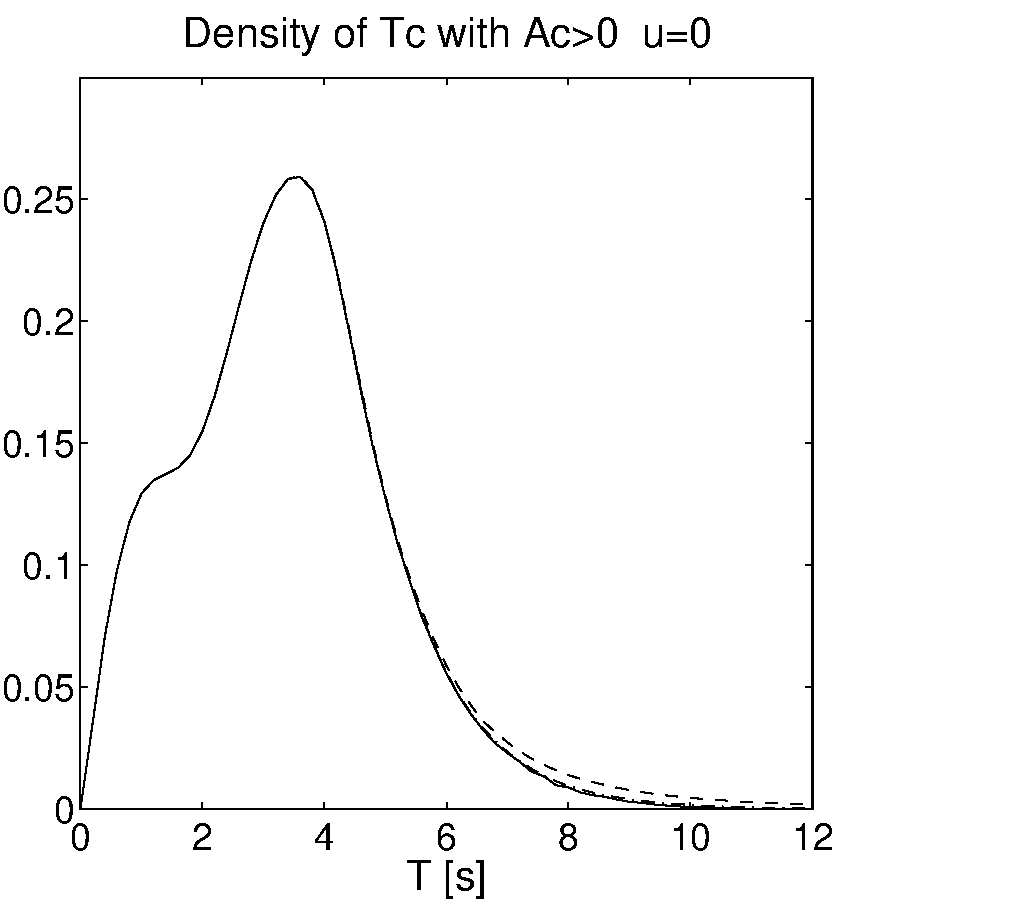
\includegraphics[width=\defwidth]{fig41a_2017}
\end{minipage}}%
\hfill
\subfigure[]{%
\begin{minipage}[b]{0.49\textwidth}%
\label{fig71b}
\centering 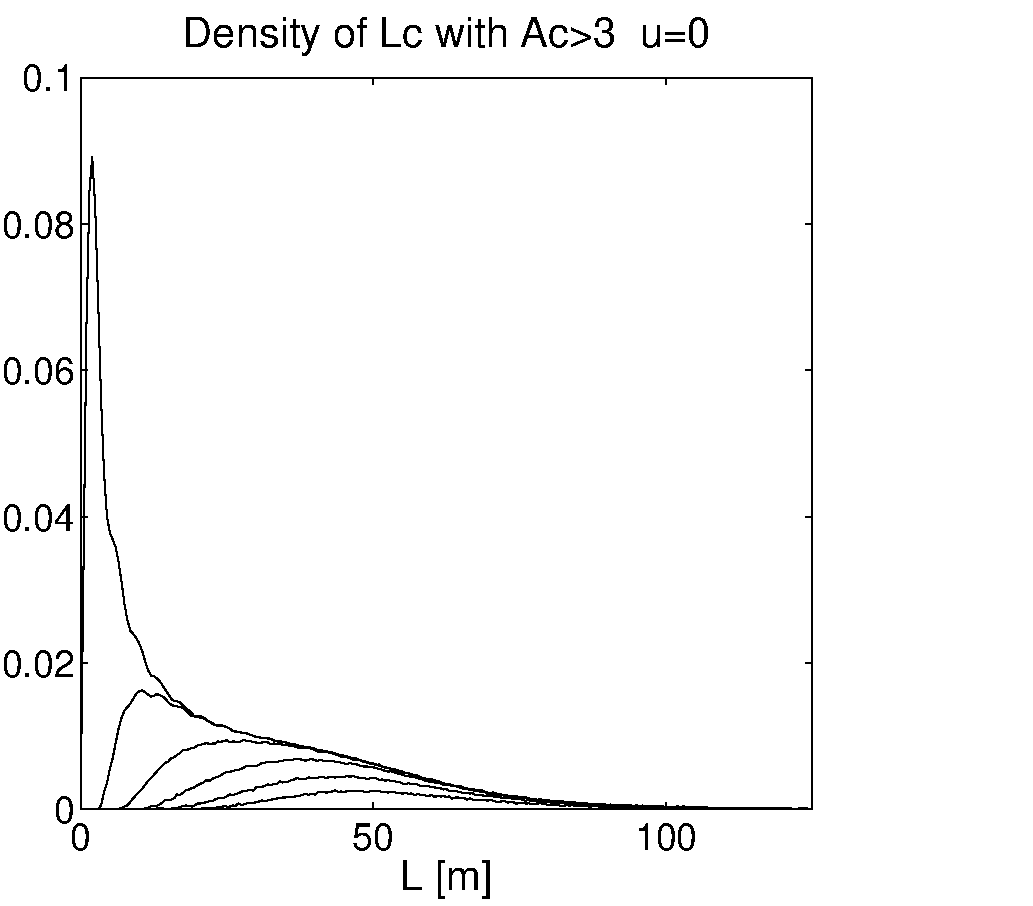
\includegraphics[width=\defwidth]{fig41b_2017}
\end{minipage}}
\vspace{-3mm}
  \caption[Density of crest period {\tt Tc} and  crest length
  {\tt Lc}]{
(a) Densities {\tt f\_tc\_1} (solid), {\tt f\_tc\_2} (dashed),
and {\tt f\_tc\_4} (dash dotted)
of crest period {\tt Tc} for Torsethaugen spectrum {\tt ST}.
(b) Densities of crest length
{\tt Lc}, (most peaked curve) compared to the density when restricted
to waves with crest height {\tt Ac} more than 10\%, 20\%, 30\%, 40\%, 50\%
of the significant wave height above the still water level,
for Gaussian sea with the Torsethaugen spectrum with {\tt Hs = 6[m]}.
Lowest curve corresponds to {\tt Ac > 3[m]}; the exact proportion is 10.2\%, 
according to Table~\ref{tab:AcCDF}.
}
  \label{fig71}
\end{figure}


The last argument in the calls above to {\tt spec2tpdf} is worth
special attention, and we will later study its effect in detail.
It controls the numerical algorithm that computes the density. Here, we
only note that a positive choice, here {\tt 4}, gives an upper bound
to the density, more accurate and more time consuming the higher the value,
while a negative value, here {\tt -1}, given an almost unbiased value in much shorter time.
\end{cex}

\subsubsection{Crest length}
\begin{cex}{Ex_Torseth}  {\sl (Crest length)} \label{pageTorsethCrestLength}
We then turn to the density of crest length for the Torsethaugen spectrum.
It can be computed using the same function {\tt spec2tpdf}, we just
change the input {\tt def} variable {\tt 'Tc'} to {\tt 'Lc'}.
{\small\begin{verbatim}
      f_Lc = spec2tpdf(ST,[],'Lc',[0 100 151],[],-1);
      pdfplot(f_Lc,'-.'), hold on
\end{verbatim}}

The crest length density has a sharp peak for very short waves
-- the wave-number spectrum is much  more broad banded than
the frequency spectrum; see \cite{LindgrenEtal1998Relation}
for a general comparison of wave period and wave length.
However, the short waves have small crests and
should be considered as 'noise' rather than as apparent waves.
Consequently, we may wish to compute the proportion of waves that have crest
higher than a certain proportion of the significant wave height, e.g.\
25\%, i.e.\ one standard deviation, \verb+Hs/4 = 1.5[m]+,
and give the density of the crest length for these waves. This can be
done by specifying an extra argument {\tt h = 1.5} in the call to \verb+spec2tpdf+.
{\small\begin{verbatim}
      f_Lc_1 = spec2tpdf(ST,[],'Lc',[0 100 151],1.5,-1);
      pdfplot(f_Lc_1)
\end{verbatim}}

Figure~\ref{fig71}(b) presents the results when the crest height is
restricted to more than 10\%, 20\%, 30\%, 40\%, 50\% of the
significant wave height. and we can see that all short
waves in fact were small. (The algorithm produces some
very small negative density values. These have been removed before
the plotting; see the following section on numerical accuracy,
Section~\ref{subsec:numerical accuracy}.)

The proportion of waves with
crests above 1.5~[m] (one standard deviation) is computed by the following commands.
{\small\begin{verbatim}
      simpson(f_Lc.x{1},f_Lc.f)
      simpson(f_Lc_1.x{1},f_Lc_1.f)
\end{verbatim}}
\noindent Taking the ratio, we can see that
more than half of the waves are small,
about 37\% of the waves have crests above 1.5~[m]. Similar calculations
for the curves in Figure~\ref{fig71}(b), give the proportions of crests
above the levels in Table~\ref{tab:AcCDF}.\index[xcmds]{{\tt spec2Acdf}}
\index[xcmds]{{\tt spec2tpdf}}
\end{cex}

\begin{table}[t]
\centerline{
\begin{tabular}{l|cccccc}
level [m] & 0.6 & 1.2 & 1.5 & 1.8 & 2.4 & 3.0 \\ \hline
proportion of crests above level & 0.607 & 0.435 & 0.367 & 0.305 & 0.191 & 0.102 \\
CDF of crest height {\tt Ac} & 0.391 & 0.563 & 0.630 & 0.693 & 0.806 & 0.895
\end{tabular}}
\caption[Crest height distribution]{Second row:
proportion of crest heights above a level, computed by {\tt spec2tpdf};
Third row: CDF of crest height computed by {\tt spec2Acdf}.}
\label{tab:AcCDF}
\end{table}

\subsubsection{Crest height}
From a statistical viewpoint the crest period distribution is uniquely defined as 
the empirical distribution of the time between  mean level upcrossings and 
the following downcrossing. It is linked to a fixed observation point and 
an ``infinite'' observation interval. Similarly, crest length distribution is 
the empirical distribution of the distance between mean level up- and downcrossings. 
It is linked to a fixed time and a fixed, ``infinitely long'', observation transect 
on the ocean surface. 
Discussing crest height distribution, the maximum height between an up- and a 
downcrossing, we obviously have to decide which observation scheme is used. 
Fortunately, the \progname{} routine {\tt spec2Acdf} handles both alternatives, 
depending on the type of spectrum we use.. 

\begin{cex}{Ex_Torseth} {\sl (Crest height)}\label{pageTorsethCrestHeight}
The table of the proportion of high crest waves is related
to the cumulative distribution function (cdf) of the crest height {\tt Ac}
in a natural way. The routine {\tt spec2Acdf} computes and plots
the cdf directly, both for the crest height over a crest period in time
and for the crest height over a crest length in space. It also plots the Rayleigh approximation. 

The following commands creates empirical and theoretical crest height distributions 
in time and in space for Gaussian waves with Torsethaugen frequency spectrum. 
The vector {\tt T} contains 100 replicates of 400 seconds of time wave simulation, the vector 
{\tt L} contains 100 replicates of 4000 meters of space wave simulation. {\tt AcT, AcL} 
are the time and space observed crest heights, respectively.  
{\small\begin{verbatim}
      clf; Hs = 6;
      r = (0:0.12:1.1*Hs)';
      F_Ac_s1_T = spec2Acdf(ST,[],'Tc',[0 12 61],r,-1); hold on
      T = spec2sdat(ST,[40000,100],0.01);
      [SteepT,HeightT,AcT] = dat2steep(T);
      plotedf(AcT,'-.')
      F_Ac_s1_L = spec2Acdf(ST,[],'Lc',[0 125 251],r,-1);
      L = spec2sdat(spec2spec(ST,'k1d'),[40000 100],0.1);
      [SteepL,HeightL,AcL] = dat2steep(L);
      plotedf(AcL,'-.')
      plot(r,1-exp(-8*r.^2/Hs^2)), hold off
\end{verbatim}}

Figure~\ref{fig:AcCDF}
shows the empirical distribution of {\tt Ac} in a long simulation in time,
and the theoretical distribution functions for crest height
in time and in space computed by {\tt spec2Acdf}, as well as the Rayleigh approximation from
Section~\ref{ss:Rayleighapproximation}. The simulations contain {\tt 9255}
space wave crests and {\tt 5823} time wave crests. The agreement between the
empirical and theoretical distribution functions is very good. 
The Rayleigh distribution gives a good approximation of the time crest height 
for large crest values but over-estimates the smallest crests. \index[xcmds]{{\tt dat2steep}}
\index[xcmds]{{\tt spec2Acdf}}\index[xcmds]{{\tt spec2spec}}
\index[xcmds]{{\tt spec2sdat}}
It does not work 
for space waves.

The third row in Table~\ref{tab:AcCDF}
shows the cdf values for crest height in space computed by {\tt spec2Acdf}.
The sum of the second and third row should be one; here, 
all sums in the table are greater than {\tt 0.997}.
\end{cex}

\begin{figure}[tbh]
\centerline{
%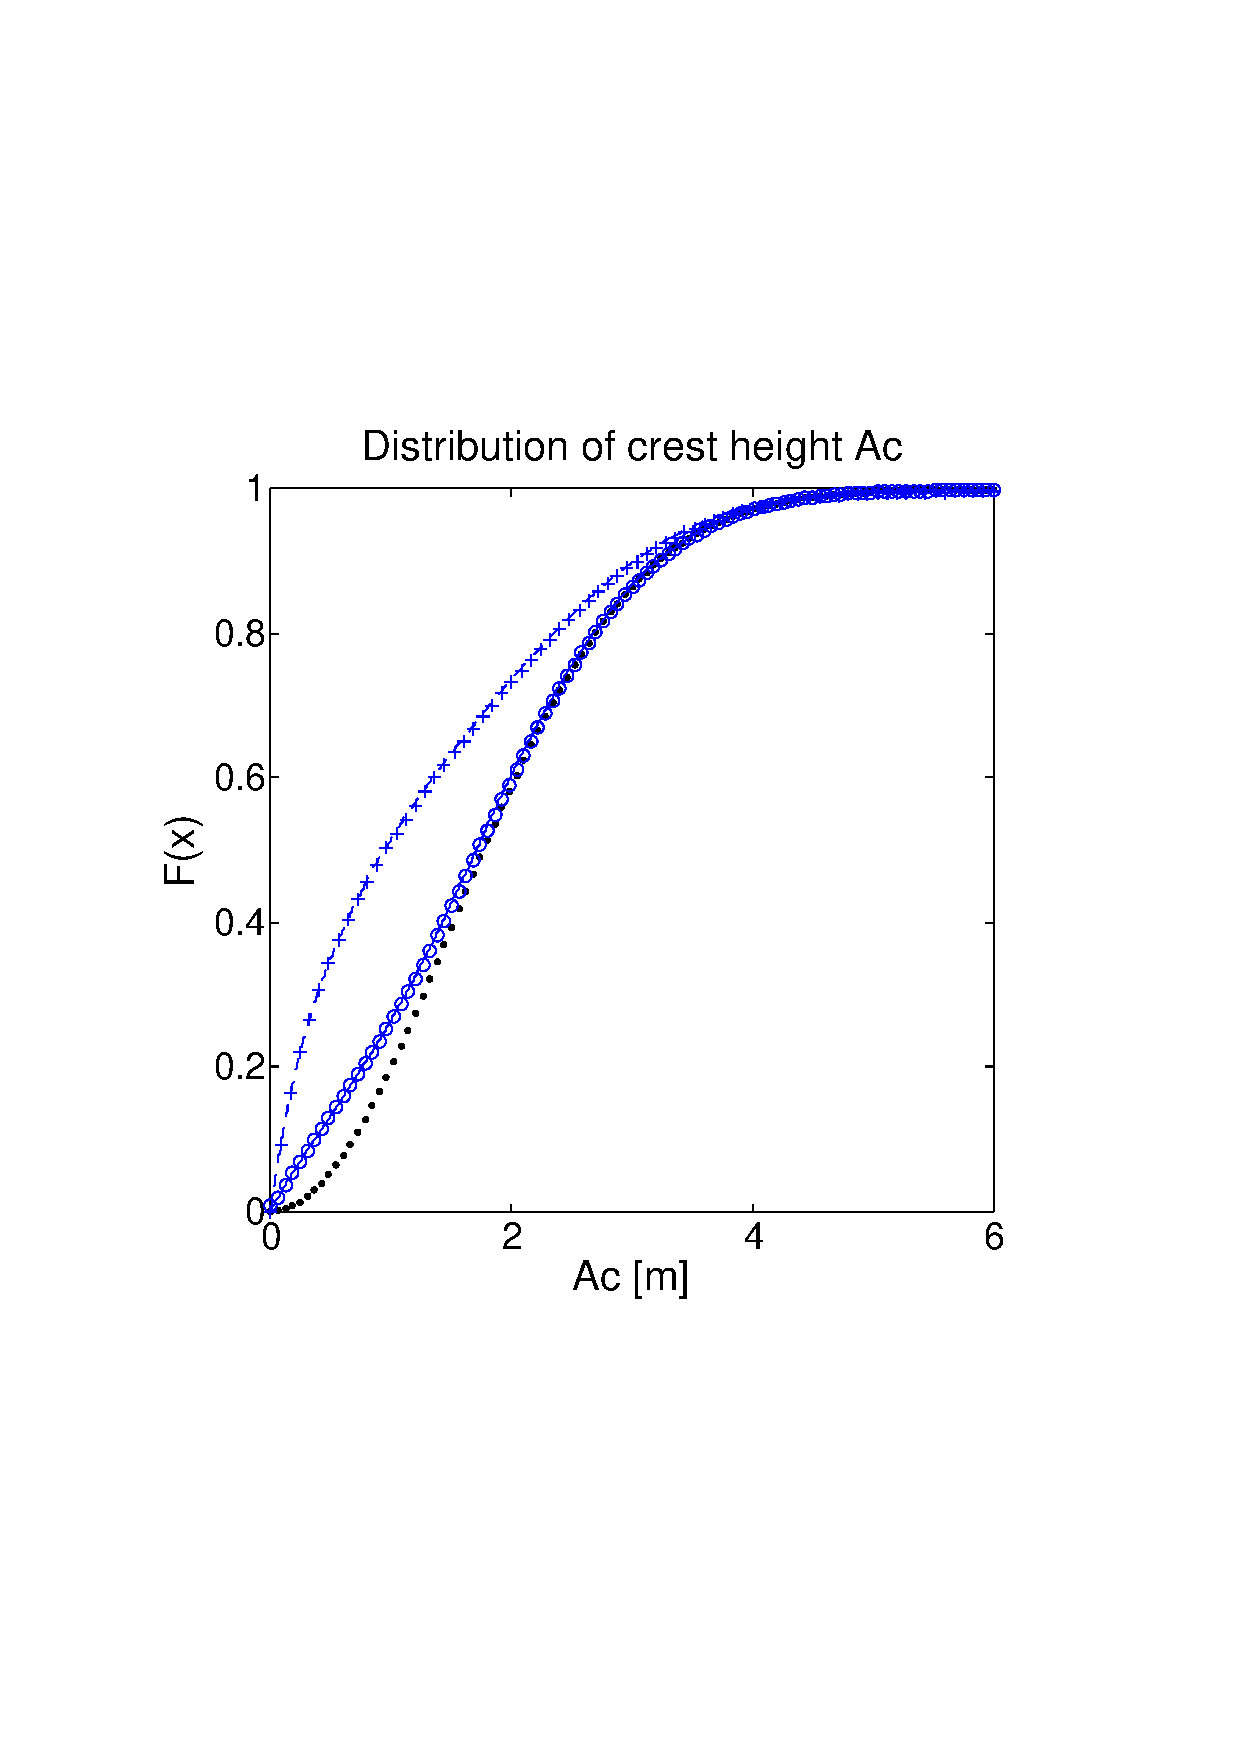
\includegraphics[height=60mm]{figAcCDF}
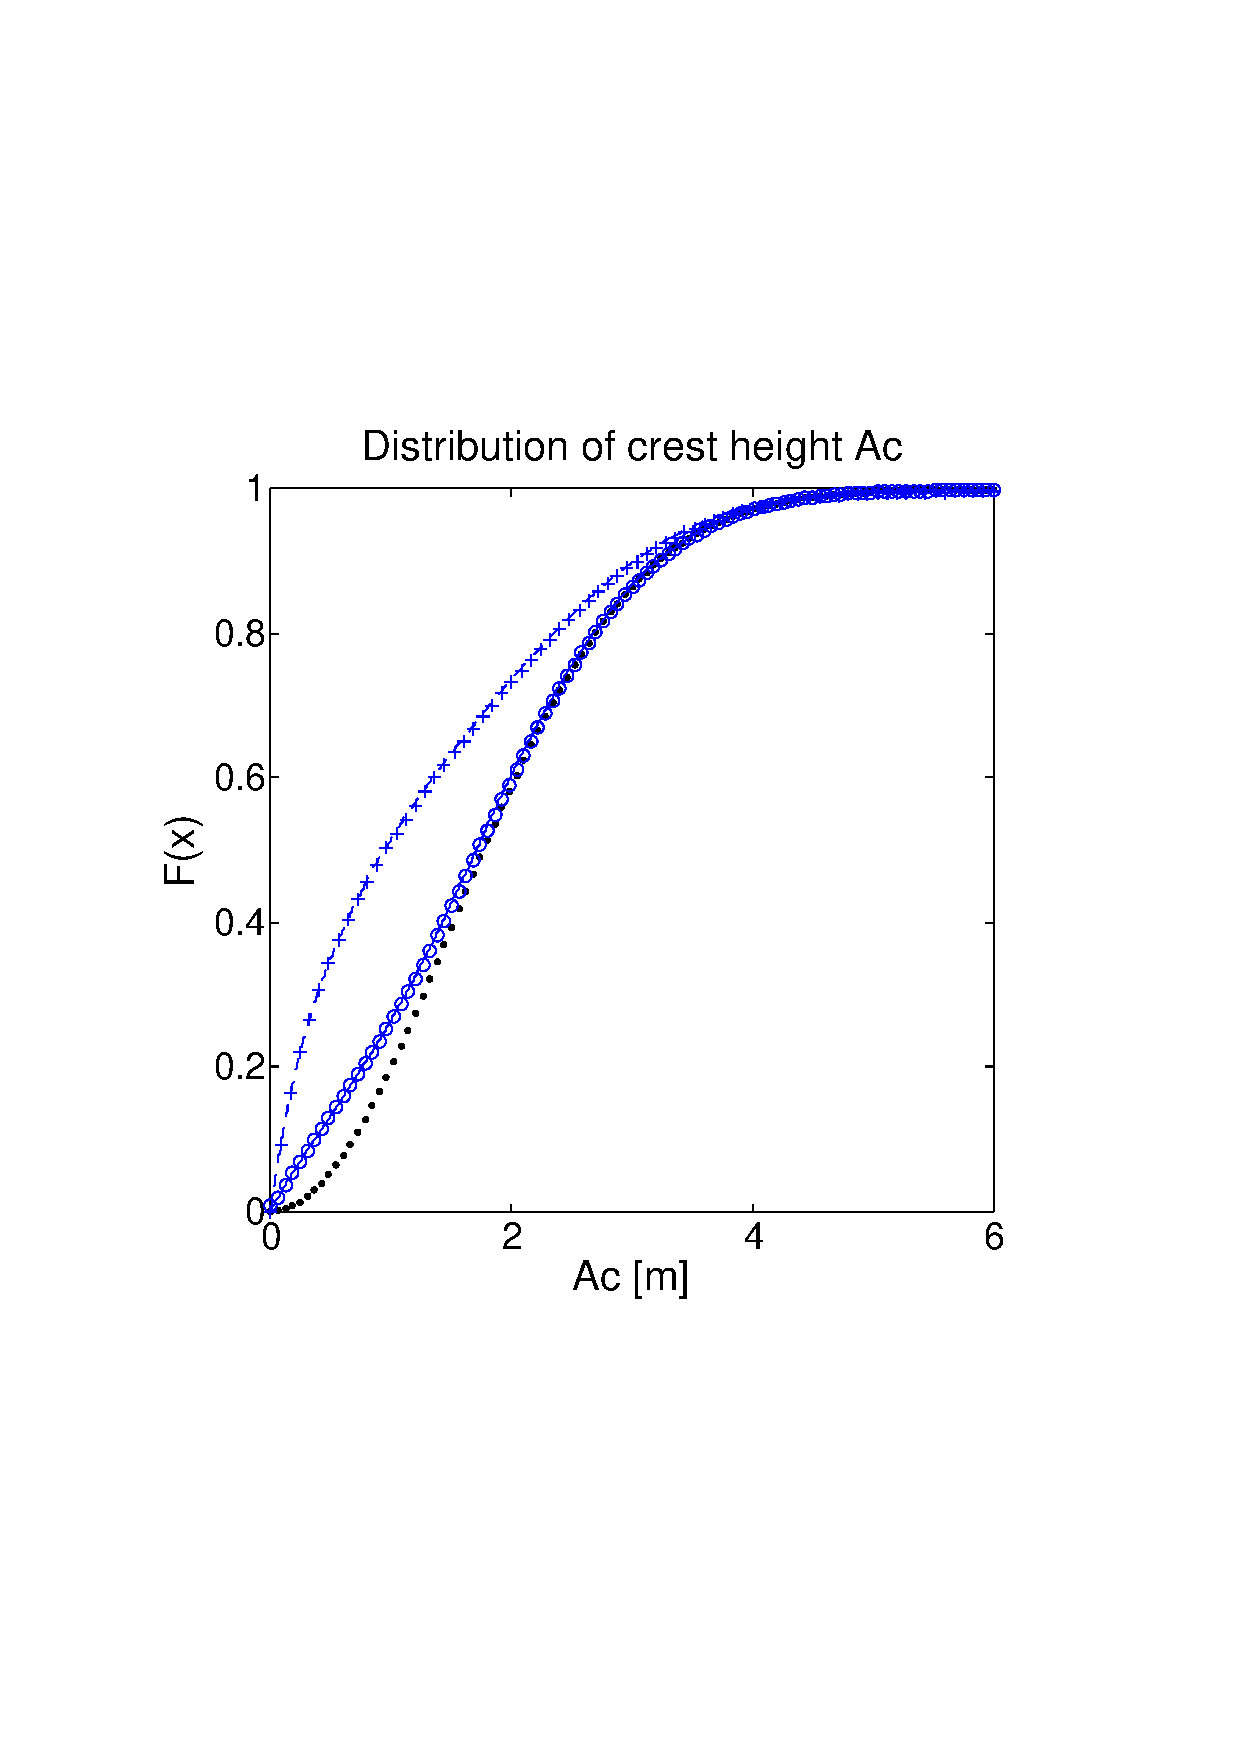
\includegraphics[width=\onefigwidth]{figAcCDF}
%\hspace{5mm}
%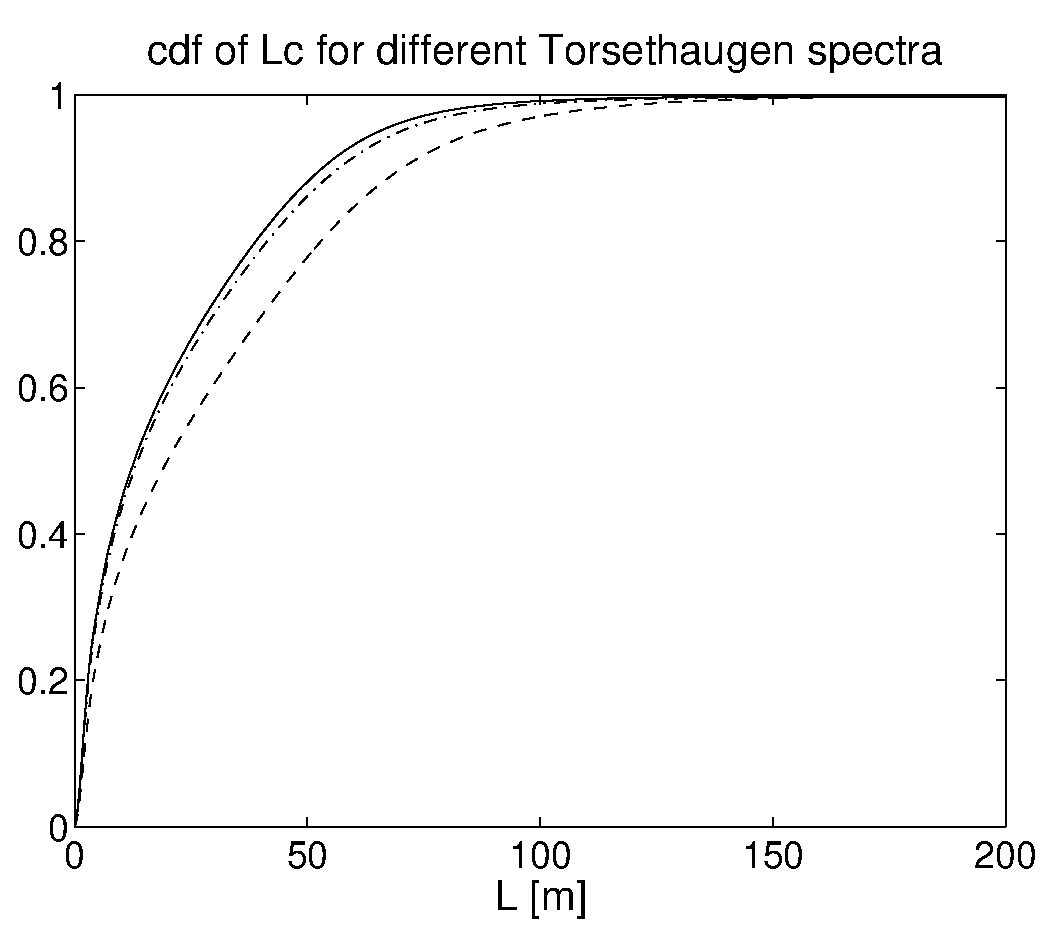
\includegraphics[height=60mm]{fig42}
}
\vspace{-3mm}
\caption[Cumulative distribution for crest height Ac]%
{Cumulative distribution (cdf) for crest height {\tt Ac}
with Torsethaugen spectrum {\tt ST}.
Curves most to the left = theoretical (solid)  and empirical
(dash dotted) cdf for {\tt Ac} over a crest length. 
Middle curves show theoretical and empirical
cdf for {\tt Ac} over a crest period. Curve most to the right 
is the cdf for the Rayleigh approximation.}
\label{fig:AcCDF}
\end{figure}

\begin{figure}[tbh]
\centerline{
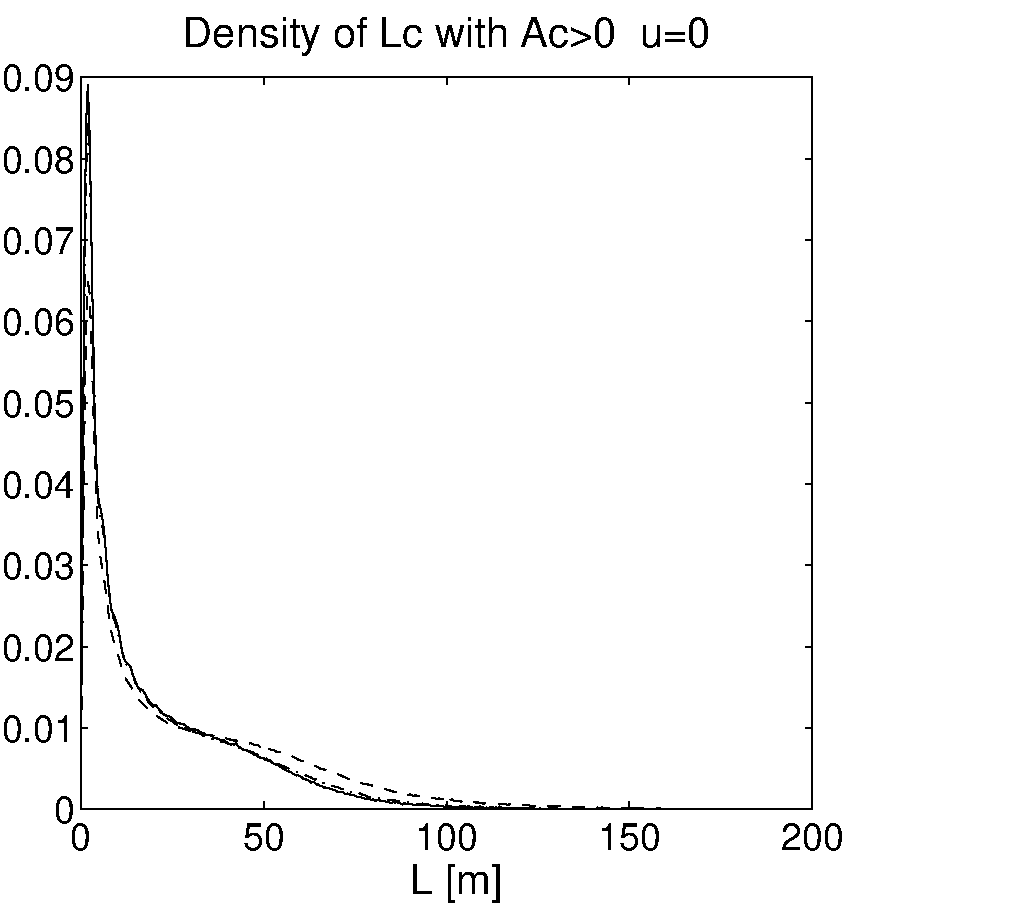
\includegraphics[height=60mm]{fig42a_2017}
\hspace{5mm}
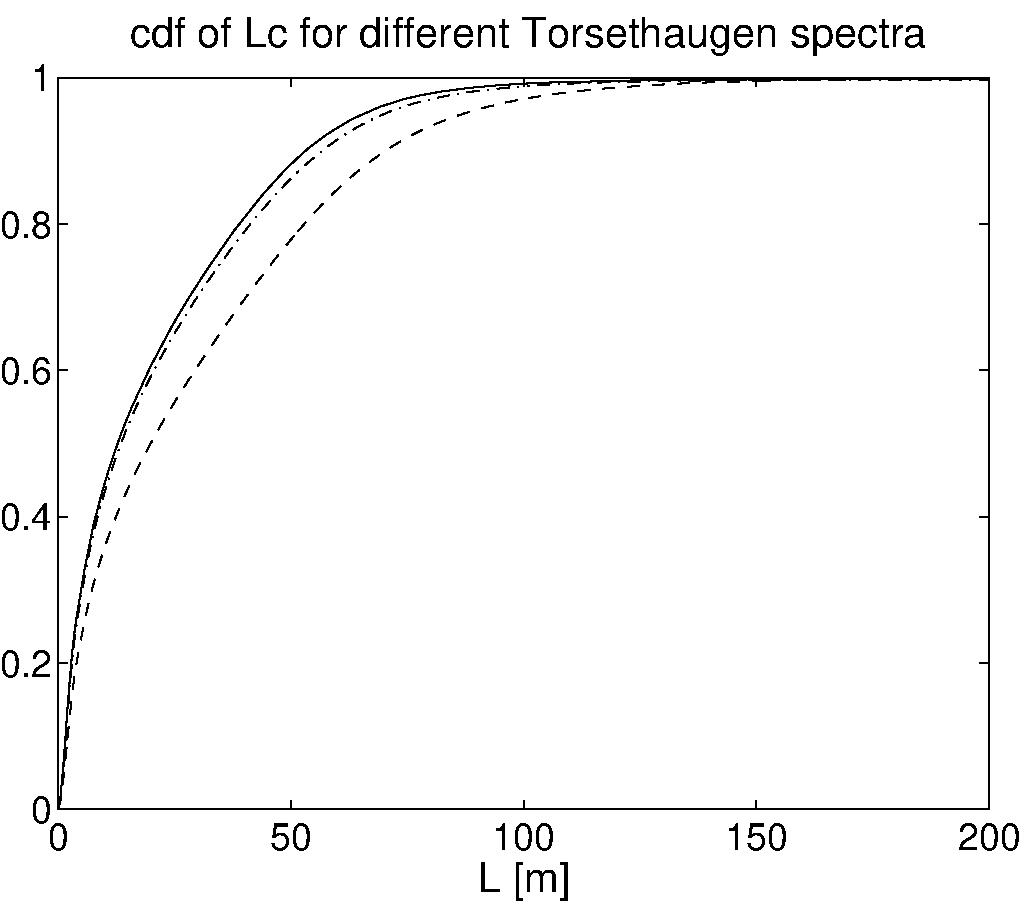
\includegraphics[height=60mm]{fig42_2017}
}
\vspace{-3mm}
\caption[Density and cumulative distribution for
{\tt Lc} with directional spreading]%
{Computed pdf (left) and cdf (right)
for {\tt Lc} in Gaussian sea with Torsethaugen
spectrum with different spreading: unidirectional spectrum {\tt S1}
(solid line) ; frequency independent spreading {\tt SD1}
(dash-dotted line); frequency dependent spreading {\tt SD12}
(dashed line).}
\label{fig:42}
\end{figure}

\begin{cex}{Ex_Torseth}{\sl (Directional spreading)} 
We finish this example by considering the Torsethaugen spectrum
with the two different spreading functions {\tt STD1} and {\tt STD12}.
In Figures~\ref{fig:00sima} and \ref{fig:00simb} we presented simulations of the sea surfaces
with these spectra. From the figures we expect that the two crest length
distributions should be different.
(Obviously, the crest period densities are identical).
In the directional sea we have to define the azimuth of the
line for which the crest length should be computed (the default value
is zero). Now, the directional spectra {\tt STD1} and {\tt STD12}
have different main wave directions, $90^o$ and $0^o$ degrees, respectively,
and hence we shall choose different azimuths for the two spectra.
More precisely, for both cases we shall consider heading waves; this
is achieved using the function {\tt spec2spec}.
{\small\begin{verbatim}
      f_Lc_d1 = spec2tpdf(spec2spec(STD1,'rotdir',pi/2),[],...
                'Lc',[0 200 201],[],-1);
      pdfplot(f_Lc_d1,'-.'), hold on
      f_Lc_d12 = spec2tpdf(STD12,[],'Lc',[0 200 201],[],-1);
      pdfplot(f_Lc_d12), hold off

      figure(2)
      dx = f_Lc.x{1}(2)-f_Lc.x{1}(1);
      dx1 = f_Lc_d1.x{1}(2)-f_Lc_d1.x{1}(1);
      dx12 = f_Lc_d12.x{1}(2)-f_Lc_d12.x{1}(1);
      plot(f_Lc.x{1},cumsum(f_Lc.f)*dx), hold on
      plot(f_Lc_d1.x{1},cumsum(f_Lc_d1.f)*dx1,'-.')
      plot(f_Lc_d12.x{1},cumsum(f_Lc_d12.f)*dx12,'--'), hold off
\end{verbatim}}

As expected, after examination of the simulated sea surfaces in
Figures~\ref{fig:00sima} and \ref{fig:00simb}, the crest length
for the two directional spectra are different.
The sea with frequency dependent spreading seems to be more irregular.
We can see in Figure~\ref{fig:42} that waves with frequency
independent spreading are only slightly
longer than the waves in unidirectional sea, while the
crest length of both seas are much shorter than for frequency
dependent spreading. 
%From Figure~\ref{fig:directspect} it is clear
%that the spectrum with frequency independent spreading function is more
%similar to the unidirectional spectrum than that with the
%frequency dependent spreading.
\end{cex}

\subsection{Numerical accuracy and computational speed}
\label{subsec:numerical accuracy}
\index[xentr]{numerical accuracy}
The basic algorithm in the routine {\tt spec2tpdf} computes a
finite-dimensional approximation to an "infinite-dimensional"
normal expectation. The last input in all the previous calls
to the routine is a parameter called {\tt nit}, and it
determines both the integration method and the dimensionality
of the computed integral.
Important references on how to compute normal probabilities are
\cite{AmbartzumianEtal1998Multinormal,Brodtkorb2004Probability,
Brodtkorb2006Evaluating,Genz1992Numerical,GenzAndKwong2000Numerical,
Rychlik1992Confidence}.

The {\tt nit} parameter can be positive, negative, and zero.
Positive {\tt nit} values use numerical, deterministic, integration
algorithms, while negative values use a simulation technique
based on importance sampling; see \cite{Brodtkorb2004Probability,
Brodtkorb2006Evaluating} for a review of different methods.

The methods with positive {\tt nit} are very reliable and have
been tested on different wave problems since the first version was
used already in 1987; see \cite{Rychlik1987Regression}. As default,
they give an upper bound to the densities.
The integration methods corresponding to negative {\tt  nit} values are
%still under tests and modifications. However, they are 
often much faster and also very accurate in cases when the
deterministic method has troubles with too long execution times;
see \cite{Lindgren2017} for examples. 

Although the method  with negative {\tt nit} is based on
simulation, the accuracy is still controlled. If the number of
simulations is too small to achieve the required accuracy
the program gives an error statement with an estimate of
the possible error in the computed density.

One should be aware that both positive and negative {\tt nit} values
can produce negative density values with {\tt spec2tpdf}. This is
the result of the way  the densities are computed, namely as differences
between "cumulative distribution type" functions. Then, small numerical
variations may cause negative density estimates, mostly for very
small density values.

The routine {\tt spec2tpdf} is the \ML{} interface to a
{\sc Fortran} program. All programs computing exact
densities of different wave characteristics
can be reformulated in such a way that the density is written as a
certain multidimensional integral of a function of Gaussian
variables; see \cite{LindgrenAndRychlik1991Slepian} for more details.
This integral is computed using a {\sc Fortran} module called
{\tt RIND}. There is also a \ML{} interface called
{\tt rind}\index[xcmds]{{\tt rind}} which can be
used to test programs for new wave characteristics.

An example is a function {\tt spec2tpdf2} which uses the program
{\tt rind}. The program is slower than {\tt spec2tpdf},
and it does not have an option that allows to choose waves with crest
above some level, but on the other hand it is easier to use for
experimentation, and it can also be used to learn how to
create own programs.

Besides the parameter {\tt nit}, the input parameter {\tt speed} will
also control the accuracy of the computations in module {\tt trgauss};
see the help text to the routines for information.

\begin{remark}
The accuracy of the numerical computations depends on the parameters {\tt nit} and {\tt speed} in 
a natural and predictable way. Of course, also the choise of  grid size affects the 
accuracy; some of the algorithms are very sensitive to short time or space steps and can 
produce covariance matrices which are not positive definite. 

\ML{} version, computer CPU, and RAM memory size, all affect speed. More subtle effects of hardware implementation 
can affect some computed small probabilities, of interest in applications. In the examples we 
present many numerical results and execution times, and the reader is advised to make own experiments 
to become familiar with these characteristics.  
\end{remark}

\begin{cex}{Ex_Torseth} {\sl (Numerical accuracy and the parameter {\tt nit})} 
We shall exemplify the use of the parameter {\tt nit} by computing the
crest length density for the directional spectrum with frequency
independent spreading.
We shall also use the slower program {\tt spec2tpdf2} for
illustration. We fix the speed and method by setting an option variable.\index[xcmds]{{\tt spec2tpdf2}}
{\small\begin{verbatim}
      opt1 = rindoptset('speed',5,'method',3);
      STD1r = rotspec(STD1,pi/2);
      f_Lc_d1_5 = spec2tpdf(STD1r,[],'Lc',[0 200 201],[],5);
      f_Lc_d1_3 = spec2tpdf(STD1r,[],'Lc',[0 200 201],[],3);
      f_Lc_d1_2 = spec2tpdf(STD1r,[],'Lc',[0 200 201],[],2);
      f_Lc_d1_0 = spec2tpdf(STD1r,[],'Lc',[0 200 201],[],0);
      f_Lc_d1_neg = spec2tpdf(STD1r,[],'Lc',[0 200 201],[],-1);
      f_Lc_d1_n4 = spec2tpdf2(STD1r,[],'Lc',[0 200 201],opt1);

      pdfplot(f_Lc_d1_5), hold on
      pdfplot(f_Lc_d1_2), pdfplot(f_Lc_d1_3)
      pdfplot(f_Lc_d1_0), pdfplot(f_Lc_d1_neg)
      pdfplot(f_Lc_d1_n4,'LineWidth',2,'-.')
      simpson(f_Lc_d1_n4.x{1},f_Lc_d1_n4.f)
\end{verbatim}}
\index[xcmds]{{\tt rotspec}}

\begin{figure}[tbh]
\subfigure[]{%
\begin{minipage}[b]{0.5\textwidth}%
\centering 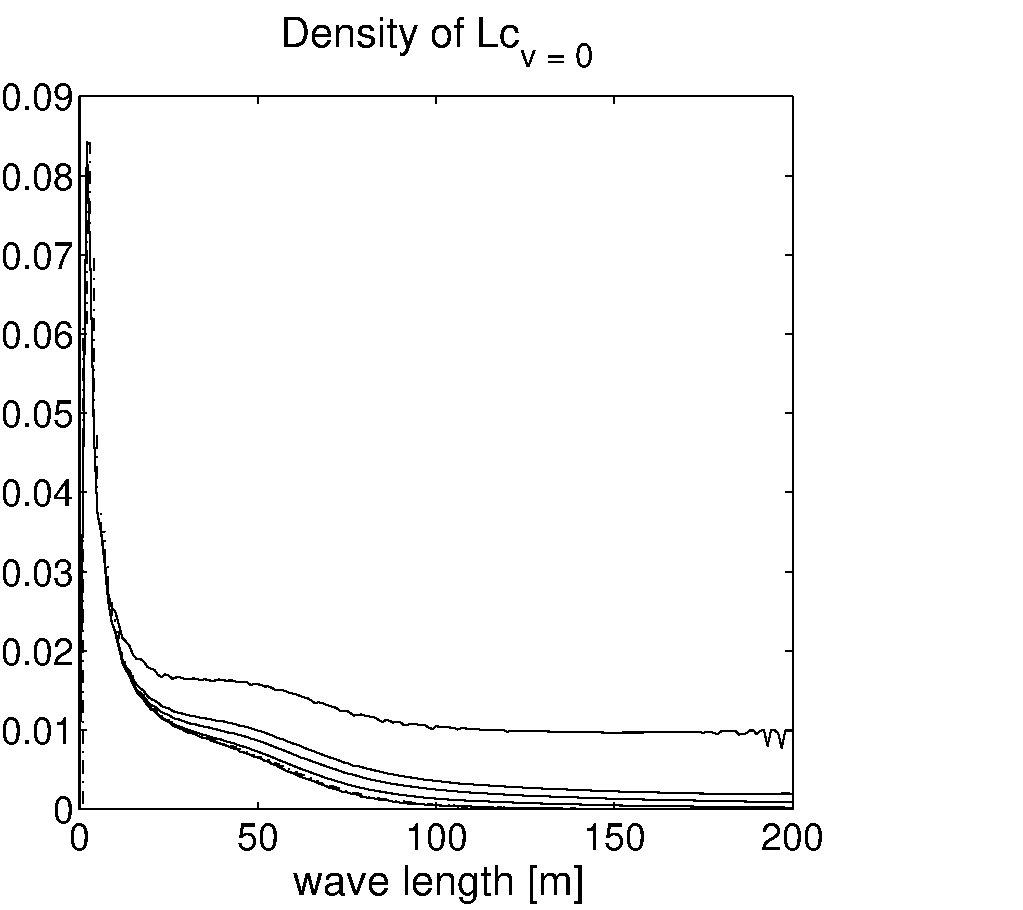
\includegraphics[height=60mm]{fig43a_2017}
\end{minipage}}%
\hfill
\subfigure[]{%
\begin{minipage}[b]{0.5\textwidth}%
\centering 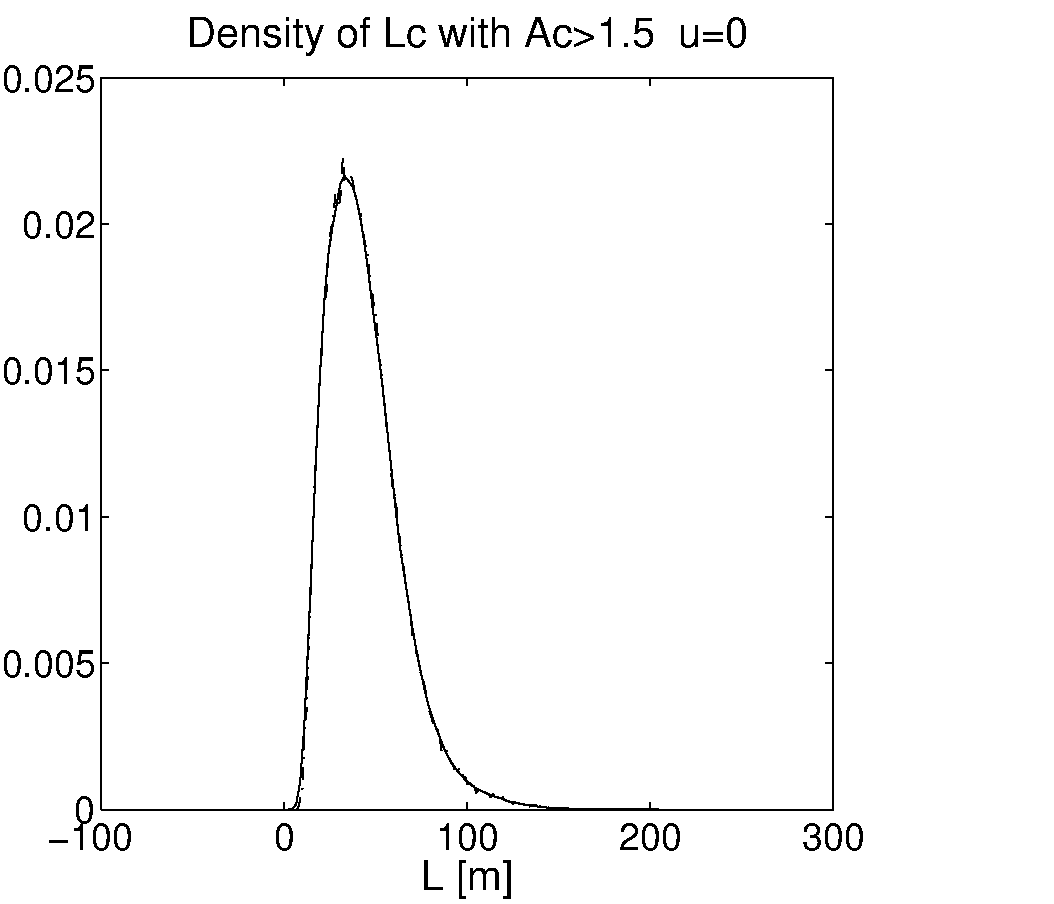
\includegraphics[height=60mm]{fig43b_2017}
\end{minipage}}
\vspace{-3mm}
  \caption[Comparison of crest length densities]{
(a) Approximations by different methods and accuracy
of the crest length for the directional
spectrum {\tt STD1r}  with frequency independent spreading.
The top solid curves are computed with
positive {\tt nit = 0 (top), 2, 3, 5}, and negative
{\tt nit = -1 (bottom)}, in routine {\tt spec2tpdf},
while the dash-dotted curve has negative
{\tt nit} with routine {\tt spec2tpdf2}.
(b) Solid curve = the empirical density of crest
length {\tt Lc} with crest height {\tt Ac > 1.5[m]},
dash-dotted curve is the
normalized computed density {\tt f\_Lc\_1}.
}
\label{fig72}
\end{figure}

The execution times for the densities were 150 seconds, 5.6 seconds, 1.3 seconds,
0.13 seconds, 2.4 seconds, and 3.7 seconds, respectively.
In Figure~\ref{fig72}(a) the different approximations are presented
and we can see how the density decreases with increasing positive {\tt nit}.
The negative {\tt nit} involves some random number integration methods,
but we can hardly see that the computed density is actually a random
function. Most problems are less numerical demanding and {\tt nit=2}
often suffices, but here clearly the negative {\tt nit} is preferable.

In Figure~\ref{fig72}(b) we compare an empirical density of crest length
{\tt Lc}, conditioned on crest height {\tt Ac > 1.5[m]}, based on 
 500~000 observed waves, with the normalized
density {\tt f\_Lc\_1} from page~\pageref{fig71}, computed with
{\tt nit = -1}. The agreement is almost perfect.
\end{cex}
\index[xentr]{wave distributions!computation of densities!
crest length and period|)}
\index[xentr]{crest!period|)}
\index[xentr]{crest!length|)}

\subsection{Wave period and wave length}

\index[xentr]{wave distributions!computation of densities!
wave length and period|(}
\index[xentr]{wave!period|(}
\index[xentr]{wave!length|(}
In the previous sections we described routines for the marginal
distributions of crest and trough periods, and height, {\tt Tc},
{\tt Tt}, {\tt Ac},  and
the corresponding crest and trough lengths, {\tt Lc}, {\tt Lt}.
We also showed how to limit the population to waves for which
the crest (trough) amplitudes are above some predetermined threshold.

We now turn to the wave period,  {\tt Tu = Tc+Tt}, which is the time
between two successive upcrossings of the still water level {\tt u}.
It is related to, but not equal to,
the crest-to-crest wave period {\tt Tcc}, which is
the time span between two successive crests. The density of {\tt Tu}
can be computed using the function
{\tt spec2tccpdf}\index[xcmds]{{\tt spec2tccpdf}}.
The wave length {\tt Lu} or encountered wave period
can also be computed by {\tt spec2tccpdf},
with just a few inputs to be modified; see the help text.
Hence, these variables shall not be discussed here any more.

The computations using {\tt spec2tccpdf} are slower than those using
{\tt spec2tpdf}, since  one needs to compute the joint density of
{\tt Tc} and {\tt Tt} and then integrate the
convolution to get {\tt Tu = Tc+Tt}. 
It should be mentioned that, in addition to the methods to reduce
computation time, one of the best methods to speed up computation is to
cut off high frequencies in the spectrum.
The syntax of {\tt spec2tccpdf} is almost identical to that of
{\tt spec2tpdf}, and hence we limit ourselves to a few examples.

\begin{rtex}{Ex_Seadatawavedistributions}{Sea data wave distributions}
In order to make comparisons with the wave characteristic
distributions in  {\tt sea.dat} we shall use the estimated spectrum \verb+SS+, see
Example~\ref{Ex_sea_statistics} on pages \pageref{Ex_sea_statistics}
and \pageref{fig2_spc}.
We first re-compute the spectrum estimate and the transformation to
Gaussianness, and extract some characteristics.

{\small\begin{verbatim}
      xx = load('sea.dat');
      x = xx;
      x(:,2) = detrend(x(:,2));
      SS = dat2spec(x);
      si = sqrt(spec2mom(SS,1));
      SS.tr = dat2tr(x);
      Hs = 4*si
\end{verbatim}}
\noindent The estimated spectrum is plotted in Figure~\ref{fig:seaspectrum},
together with pointwise 95\% confidence intervals. 

Note that the spectrum contains a transformation 
field {\tt SS.tr}, and recall the {\sc Important note 1} on page~\pageref{ImpNote_1}. 
If you want to simulate new versions of {\tt sea.dat} by {\tt spec2sdat} you must 
normalise the spectrum to have $m_0 = 1$.
\end{rtex}

\begin{figure}[tbh]
\centerline{
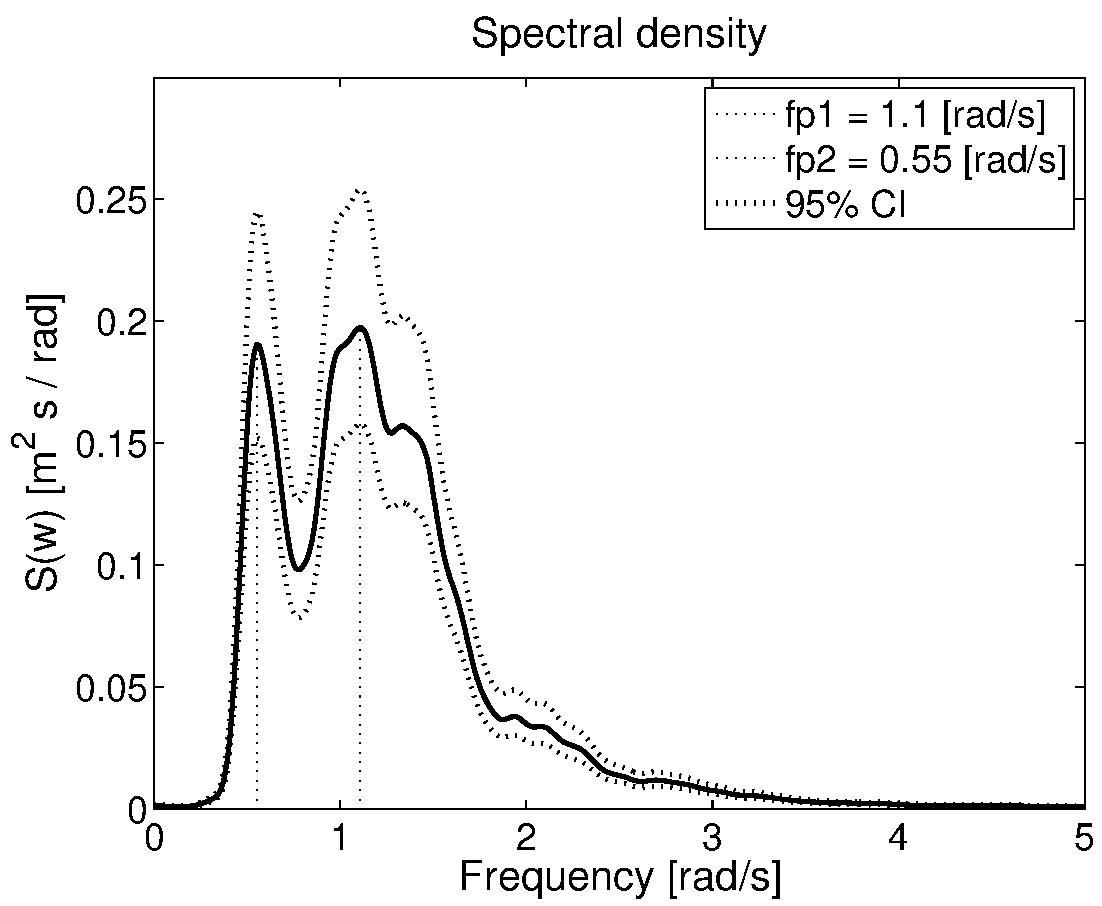
\includegraphics[width=\narrowfigwidth]{seaspectrum}
}
\vspace{-3mm}
\caption[Estimated sea spectrum]{Estimated spectrum {\tt SS} for data
{\tt sea.dat} with confidence bands.}
\label{fig:seaspectrum}
\end{figure}

\begin{cex}{Ex_Seadatawavedistributions}{\sl (Crest period)} 
We first consider the crest period,
as we did in Example~\ref{Ex_Torseth} 
on page \pageref{pageTorsethCrestPeriod}, and also the proportion of
crests with \label{page:Ex7a}
significant crest height, i.e.\ {\tt Tc} when {\tt Ac > Hs/2}, in the same way as we did for crest length.
 %in Example~\ref{Ex_Torseth} 
%on page~\pageref{pageTorsethCrestLength}. 
After that we
will do the same for wave period and consider {\tt Tu} when {\tt Ac > Hs/2}.
The proportion of crest periods with significant crest height should be the
same as the proportion of wave periods with significant crest height,
i.e.\ {\tt Tu} when {\tt Ac > Hs/2}. 
The difference between the two proportions gives an indication of 
the accuracy in the computation of the convolution {\tt Tu = Tc + Tt}.

We can also compare the calculated proportion of significant crests
with the proportion observed in data and with the approximative
Rayleigh model. Finally, we estimate the density using KDE from data
and compare to the theoretically computed one, based on the transformed
Gaussian model. \index[xcmds]{{\tt kde}}

For completeness we again estimate the transformation and find wave
characteristics in the signal. The crest period, {\tt Tc}, distribution,
estimated from data, and the computed density are almost identical,
except for very short waves; see Figure~\ref{fig73}(a), obtained by
the following commands. Note the last output variable 
{\tt yn} in the call to {\tt dat2steep}, which
is an interpolated series, to be used later, when we need more exact values 
for the wave periods.\label{Interpol_yn}
{\small\begin{verbatim}
      method = 0; rate = 2;
      [S,H,Ac,At,Tcf,Tcb,z_ind,yn] = dat2steep(x,rate,method);
      Tc = Tcf+Tcb;
      t = linspace(0.01,8,200);
      f_tc1emp = kde(Tc,{'L2',0},t);
      pdfplot(f_tc1emp), hold on
      f_tc1 = spec2tpdf(SS,[],'Tc',[0 8 81],0,4);
      Chk1 = simpson(f_tc1.x{1},f_tc1.f) %Integral should be one
      pdfplot(f_tc1,'-.'), hold off
\end{verbatim}}

We next compute the density of crest period,
but now for waves with significant crest height, i.e.\ waves for
which {\tt Ac > Hs/2}. In the following call to
{\tt spec2tpdf} the restriction to {\tt Ac > Hs/2} is
indicated by the argument~\verb+[Hs/2]+.
{\small\begin{verbatim}
      nit = 4;
      f_tc2 = spec2tpdf(SS,[],'Tc',[0 8 81],[Hs/2],nit);
      Pemp = sum(Ac>Hs/2)/sum(Ac>0) 
      			  %Observed proportion of high crests
      Chk2 = simpson(f_tc2.x{1},f_tc2.f) 
      			  %Integral should be equal to probability of high crests
      index = find(Ac>Hs/2);
      f_tc2emp = kde(Tc(index),{'L2',0},t);
      f_tc2emp.f = Pemp*f_tc2emp.f;
      pdfplot(f_tc2emp), hold on
      pdfplot(f_tc2,'-.'), hold off
\end{verbatim}}

The observed frequency of significant crests, {\tt Pemp = 0.1778} is 
close to the theoretically computed values, {\tt Chk2 = 0.1802} with {\tt nit = 5} and 
{\tt Chk2 = 0.1816} with {\tt nit = 4},
obtained with computation times of 18~seconds and 4~seconds, respectively. 
A finer grid, {\tt [0 8 161]} instead of {\tt [0 8 81]} in \verb+f_tc2+, will give an 
almost exact agreement with the empirical frequency with four times the computation time. 

Observe that the Rayleigh approximation would give a
probability equal to 0.1353. This is not surprising since crests in
non-Gaussian sea tend to be higher than those in Gaussian sea.

Clearly, by changing the input {\tt Hs/2} to any other fixed level
{\tt h}, and integrating the resulting density we obtain
approximations to the probability {\tt P(Ac > h)}.
When {\tt h} is a vector then it is more efficient to use the program
{\tt spec2Acdf}\index[xcmds]{{\tt spec2Acdf}} to compute {\tt P(Ac > h)},
as in the crest height Example~\ref{Ex_Torseth} 
on page~\pageref{pageTorsethCrestHeight}. 
However, before using the
program it is important to first use {\tt spec2tpdf} and check that the
computed density integrates to one. If not, the inputs {\tt param} and
{\tt nit} have to be changed. Note that the integral {\tt Chk1} is slightly 
greater than one. 

\begin{figure}
\subfigure[]{%
\begin{minipage}[b]{0.5\textwidth}%
%\centering 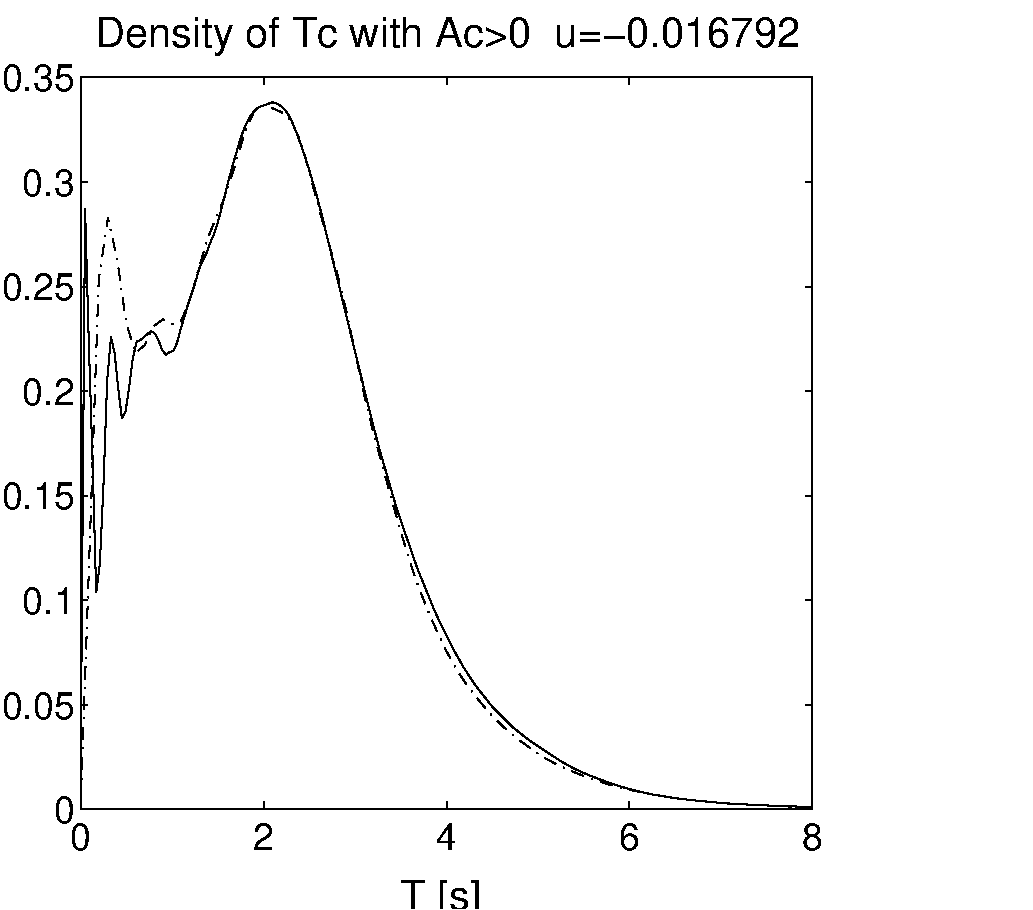
\includegraphics[width=\defwidth]{fig7_tb_2017}
\centering 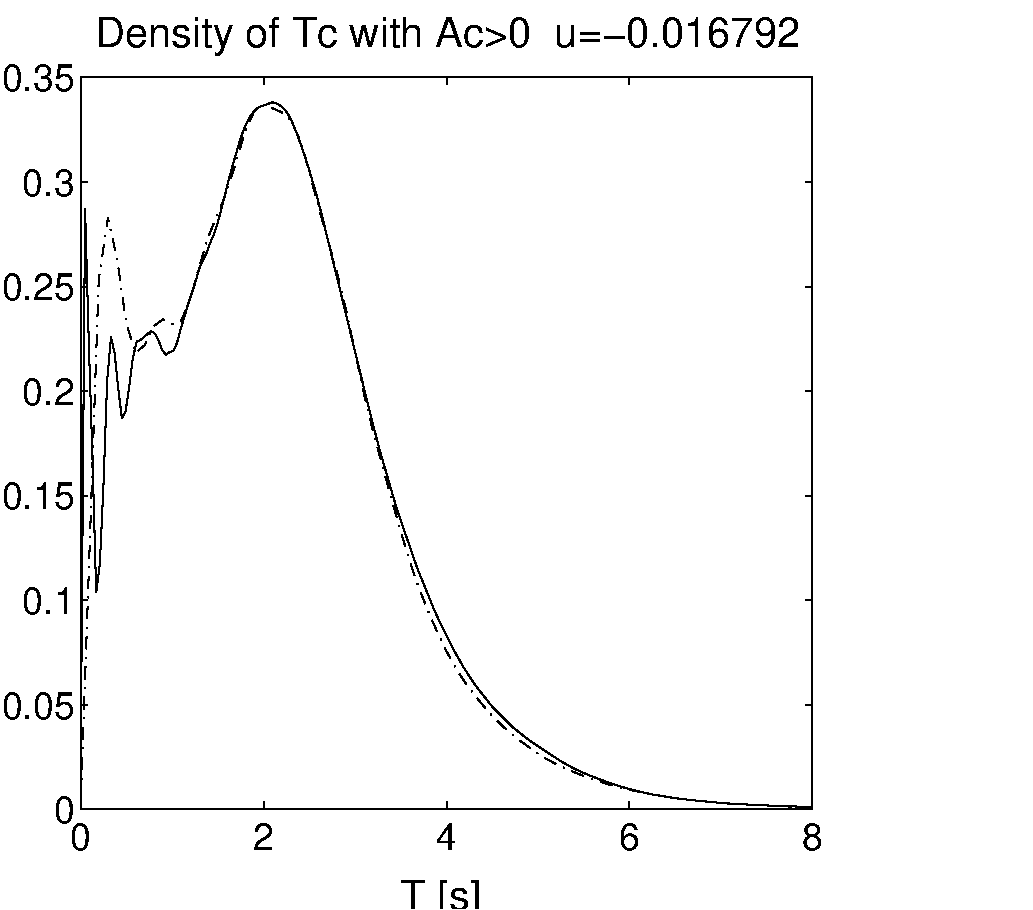
\includegraphics[height=60mm]{fig7_tb_2017}
\end{minipage}}%
\hfill
\subfigure[]{%
\begin{minipage}[b]{0.5\textwidth}%
%\centering 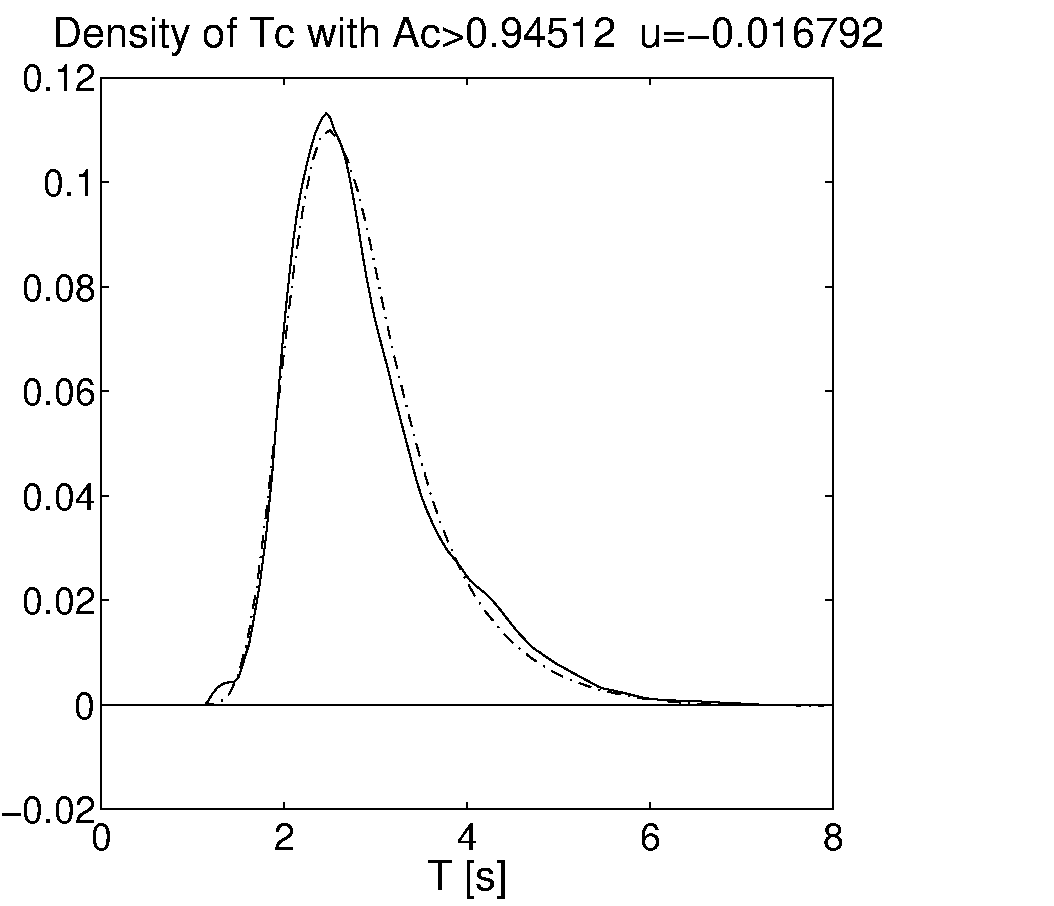
\includegraphics[width=\defwidth]{fig7_t2b_2017}
\centering 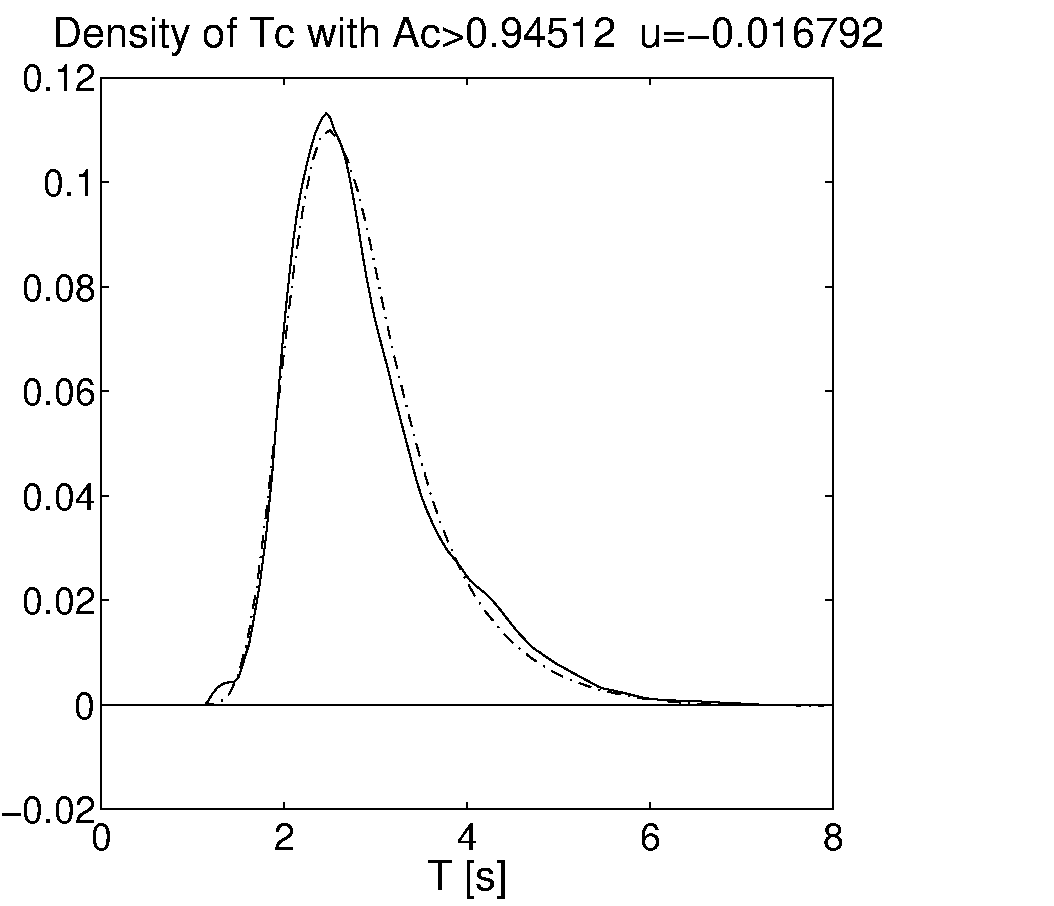
\includegraphics[height=60mm]{fig7_t2b_2017}
\end{minipage}}
\vspace{-3mm}
  \caption[Estimated and theoretical
density of crest periods in {\tt sea.dat}]{
(a) Estimated density (KDE) of crest periods in {\tt sea.dat} (solid line)
compared with theoretically
computed using {\tt spec2tpdf} (dashed line). (b) The same for the
waves with significant crest, i.e.\ {\tt Ac > Hs/2}.
}
\label{fig73}
\end{figure}

Observe that in this section we are analysing apparent waves
in time. If the input {\tt 'Tc'} in {\tt spec2tpdf} is replaced by
{\tt 'Lc'}, then we would consider waves in space and the proportion
of significant crest would probably be very different.
\end{cex}

\begin{cex}{Ex_Seadatawavedistributions}{\sl (Wave period for high-crest waves)}
We turn now to the more difficult problem of wave
period {\tt Tu = Tc+Tt}, and compute the density for 
waves with significant crest height, {\tt Ac > Hs/2} and
with {\tt At > 0}. As mentioned, this differs from crest period 
Example~\ref{Ex_Torseth} on page~\pageref{pageTorsethCrestPeriod} 
in that it involves the
distribution of the sum {\tt Tc + Tt} of two dependent random variables,
with the same marginal distribution. Since the computations need to be
done with high accuracy (the computed density is different for the
unconditional wave period and for the period of waves with crest below a given
threshold),  % see \cite{BIOPR00} for more detailed discussion),
we need to use a high positive {\tt nit} value, so that the total sum
of the density is close to 0.1789, or use a negative {\tt nit}. 
We begin with negative {\tt nit}, which gives faster results
very close to the true density, and then take {\tt nit = 3}.
{\small\begin{verbatim}
      f_tun = spec2tccpdf(SS,[],'t>',[0 12 61],[Hs/2],[0],-1);
      simpson(f_tun.x{1},f_tun.f)
      f_tu3 = spec2tccpdf(SS,[],'t>',[0 12 61],[Hs/2],[0],3,5);
      simpson(f_tu3.x{1},f_tu3.f)
      pdfplot(f_tun), hold on
      pdfplot(f_tu3,'--'), hold off
\end{verbatim}}

\begin{figure}[tbh]
\subfigure[]{%
\begin{minipage}[b]{0.5\textwidth}%
\centering 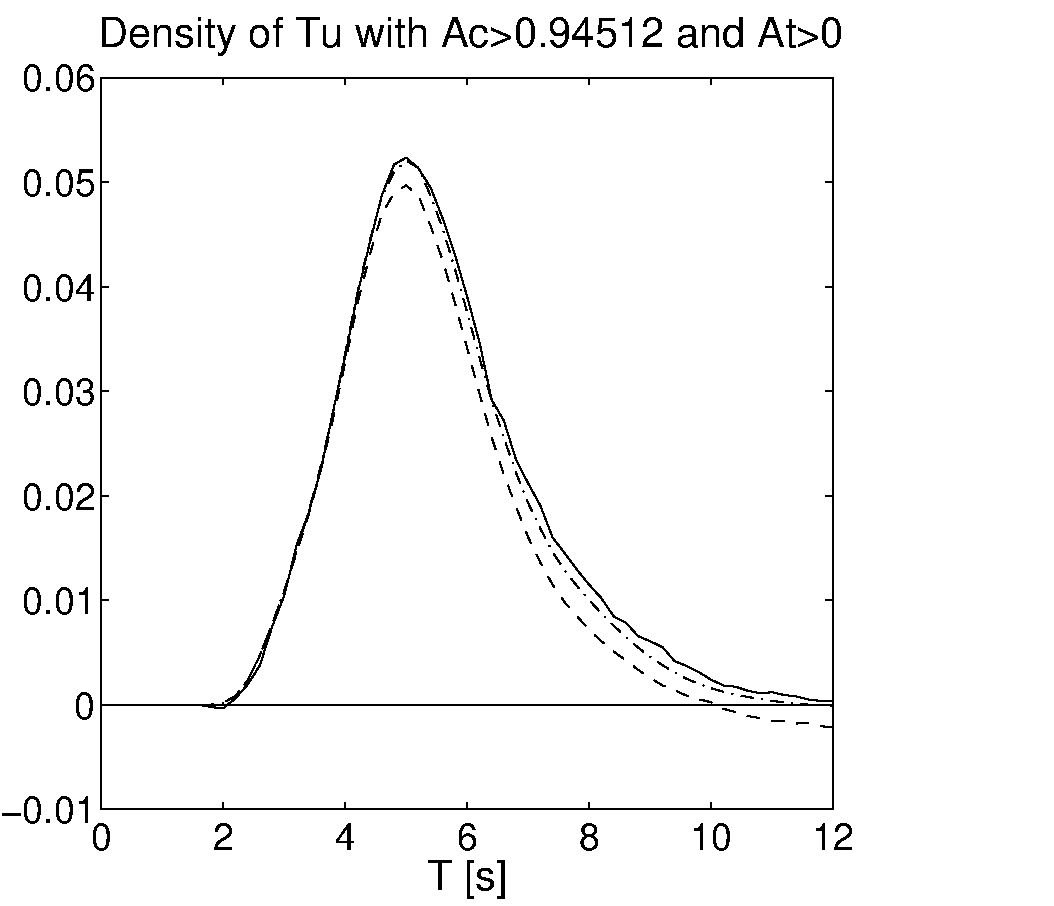
\includegraphics[height=60mm]{fig7_tcc2b_2017}
\end{minipage}}%
\hfill
\subfigure[]{%
\begin{minipage}[b]{0.5\textwidth}%
\centering 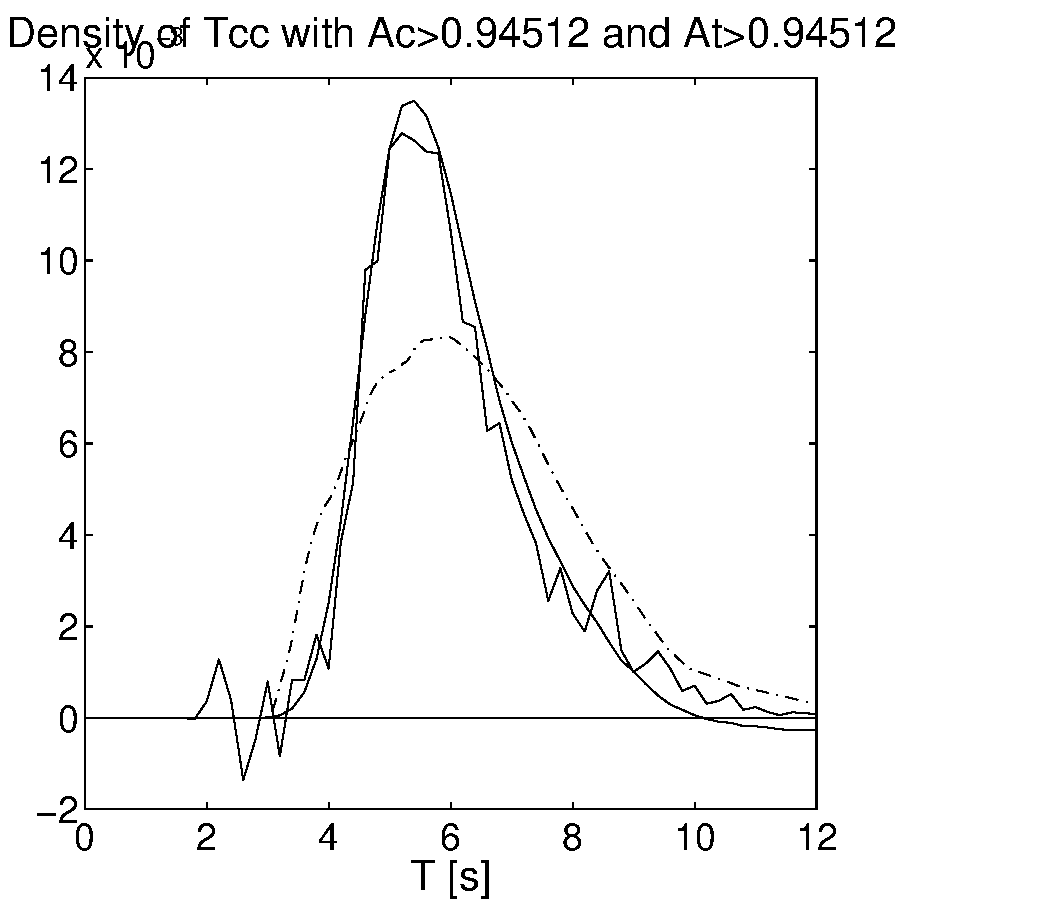
\includegraphics[height=60mm]{fig7_tcc22_4b_2017}
\end{minipage}}
\vspace{-3mm}
  \caption[Densities of period {\tt Tu}]{
(a) Densities of upcrossing period {\tt Tu} for waves with significant crest in
the transformed Gaussian  model
for {\tt sea.dat} computed with different degree of
accuracy; (solid line)  {\tt nit=-1}; the dashed line is
computed with {\tt nit=5} and the dash dotted line with {\tt nit=3}.
(b) Densities of period {\tt Tu} for waves with significant crest and
trough in the same model; solid wiggled line {\tt nit=-1}; solid smooth line
 {\tt nit=4}; the dash dotted line is estimated from
 the data with KDE.
}
 \label{fig74}
\end{figure}
The integral of the density \verb+f_tcn+ is 0.1778,
which is close to the previously computed value 0.1789.
However, the execution time was 66 seconds, compared to
21~seconds for \verb+f_t2+. The choice {\tt nit=3} takes 3~minutes
and give the integral 0.15. We have checked the program with
{\tt nit=5} (execution times 66~minutes), and the integrals was 0.17.
The densities are shown in Figure~\ref{fig74}(a). We can see that
the density computed using {\tt nit=-1} (dash-dotted line) is quite
accurate, even if it slightly
wiggly, being a random function with very small variance, and errors
compensate each other giving almost perfect total probability mass.
Note that another call of the program would give slightly different
values and the total mass would also be changed.
\end{cex}

\begin{cex}{Ex_Seadatawavedistributions}{\sl (Wave period for high-crest, deep-trough waves)}
We finish the example with an even more
interesting case, the density of wave period of waves with both
significant crest and significant trough, i.e.\ really big waves.
We  first estimate the probability of such waves in the data; then we
use the interpolated series {\tt yn} from page~\pageref{Interpol_yn}.
{\small\begin{verbatim}
      [TC tc_ind v_ind] = dat2tc(yn,[],'dw');
      N = length(tc_ind);
      t_ind = tc_ind(1:2:N);
      c_ind = tc_ind(2:2:N);
      Pemp = sum(yn(t_ind,2)<-Hs/2 && ...
             yn(c_ind,2)>Hs/2)/length(t_ind)
      ind = find(yn(t_ind,2)<-Hs/2 && yn(c_ind,2)>Hs/2);
      spwaveplot(yn,ind(2:4))
      Tu = yn(v_ind(1+2*ind),1)-yn(v_ind(1+2*(ind-1)),1);
      t = linspace(0.01,14,200);
      f_tu2_emp = kde(Tcc,{'L2',0},t);
      f_tu2_emp.f = Pemp*f_tu2_emp.f;
      pdfplot(f_tu2_emp,'-.')
\end{verbatim}}
\index[xcmds]{{\tt spwaveplot}}

The probability is estimated to be
\verb+Pemp = 0.0370+, which is slightly higher
than what we could expect if high crests and low troughs occur
independently of each other (the probability would then be less than 0.025).

We turn now to computation of the probability using {\tt spec2tccpdf}
with {\tt nit=-1}. However, we are here in a situation when the
error in computations is of the order $10^{-3}$, which is comparable
to the values of the density itself. Hence the computed function
will look very noisy.
{\small\begin{verbatim}
      f_tu2_n = spec2tccpdf(SS,[],'t>',[0 12 61],[Hs/2],[Hs/2],-1);
      simpson(f_tu2_n.x{1},f_tu2_n.f), hold on
      pdfplot(f_tu2_n), hold off
\end{verbatim}}

The execution time is less than one minute, and the
computed probability with \verb+nit = -1+ is 0.0358,
which is well in agreement with the number estimated from data. 
The more time-demanding \verb+nit = 4+ gives a much smoother 
pdf curve with almost the same integral, with an execution time of 15~minutes.

\index[xentr]{wave distributions!computation of densities!
wave length and period|)}
\index[xentr]{wave!period|)}
\index[xentr]{wave!length|)}

In Figure~\ref{fig74}(b) we see the computed densities of wave
period for these big waves. Those are well concentrated around the
mean value. It is also compared to the KDE estimator. We have not tried to
tune up the estimator that is based on only 20 values and hardly can
be considered as accurate.\end{cex}

\section{Joint density of crest period and crest
  height}\label{sec:joint_crest_period_and_height}
\index[xentr]{wave distributions!computation of densities!
joint crest height/period|(}

In this section we shall present programs for joint characteristics
of apparent waves. We shall be mostly concerned with crest period,
crest position, and crest height. Since we also want to compare the
theoretically derived densities with observations we wish to study
a longer record of measurements than we did in the previous section.
By doing so we will have more reliable statistical estimates of
the densities, but on the other hand we face the problem that the
sea state can change during the measured period -- the process is
simply not stationary.

The data come from the Gullfaks C platform, see
Figure~\ref{fig7northsea}(a). See the help text of {\tt gfaksr89}
for a detailed description of the data  and {\tt northsea}
for the instructions how the map showing location of
the platform was drawn. \index[xcmds]{{\tt gfaksr89}}
\index[xcmds]{{\tt northsea}}\index[xentr]{Gullfaks C platform}

\begin{figure}[htbp]
\subfigure[]{%
\begin{minipage}[b]{0.45\textwidth}%
\centering 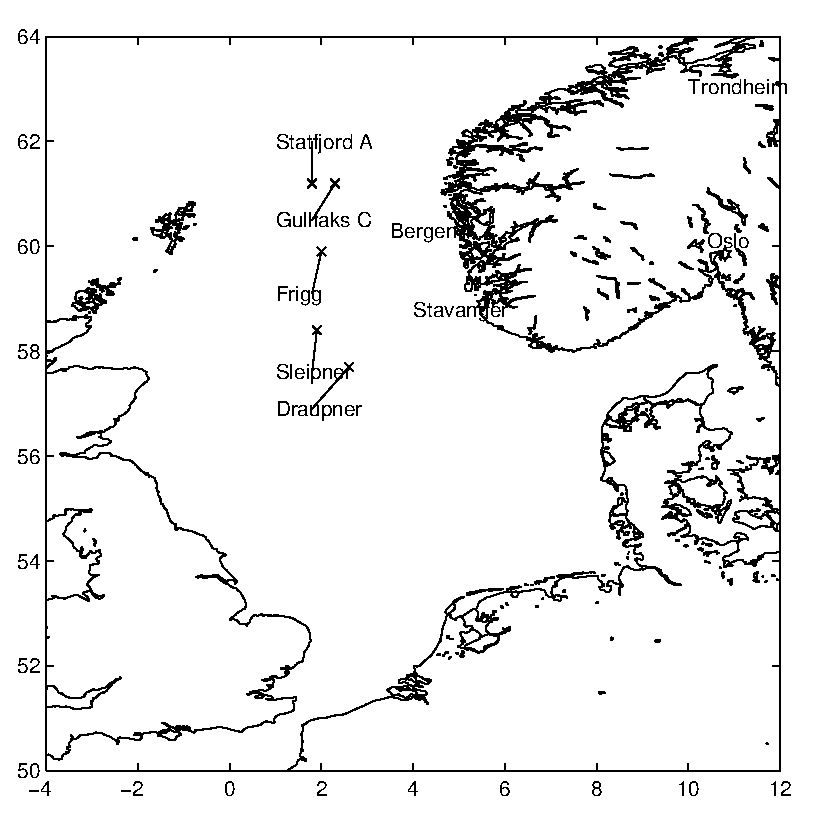
\includegraphics[height=60mm]{fig7northsea}
\end{minipage}}%
\hfill
\subfigure[]{%
\begin{minipage}[b]{0.55\textwidth}%
\centering 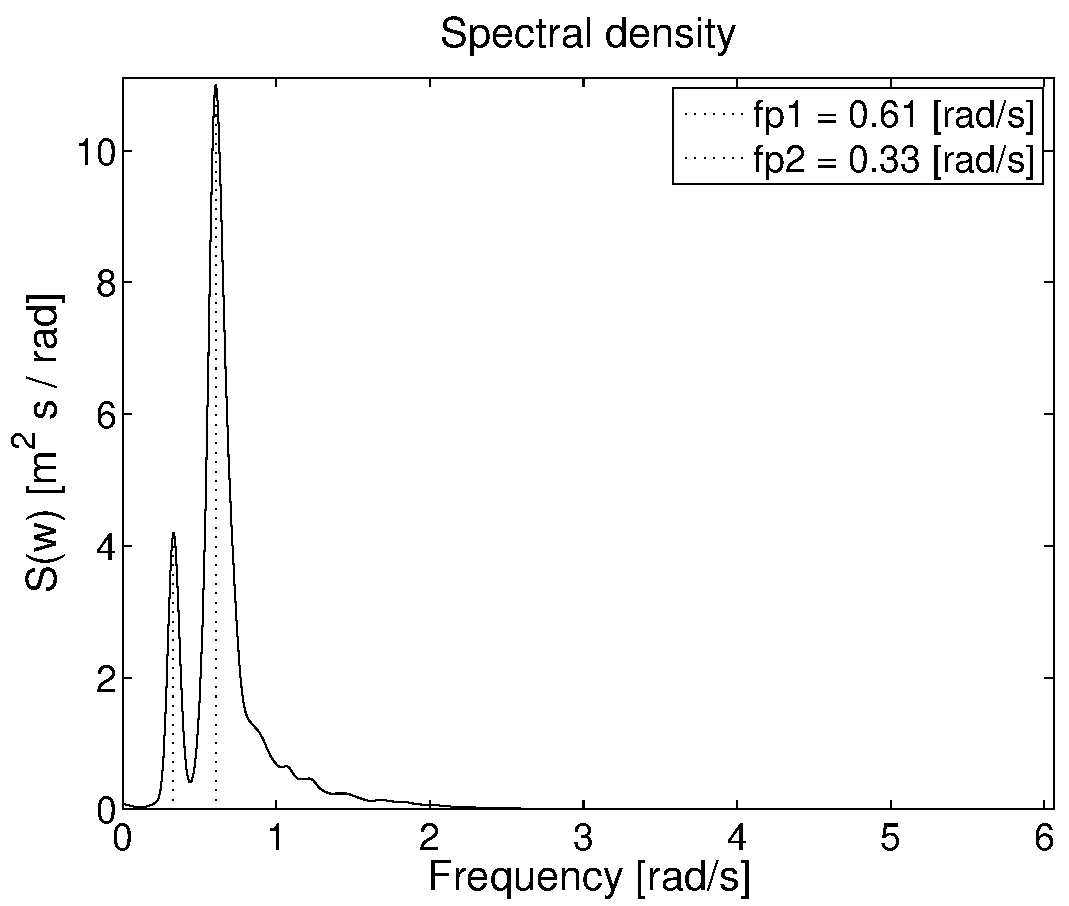
\includegraphics[height=60mm]{fig7northsea_s}
\end{minipage}}
\vspace{-3mm}
  \caption[Location of Gullfaks C platform and estimated spectrum]
{Location of Gullfaks C platform (a). The estimated spectrum (b).
}
 \label{fig7northsea}
\end{figure}

\bigskip
\noindent
{\bf WARNING:} In the following examples we run the programs with
maximum accuracy and hence we have long execution times.
Usually one should use simpler and faster approximations at first
experiments with complicated distributions. When one is satisfied with the
results, one should compute the densities
with the desired high accuracy. For testing own problems  we recommend
to start execution of programs with input parameter {\tt speed = 9,8}
(maximal speed is {\tt 9}, the default is {\tt 4}) and {\tt nit = -1, 1},
(default is {\tt 2}).
These choices will produce fast but still useful approximations.

\subsection{Preliminary analysis of data}
\begin{rtex}{Ex_preliminary_analysis}{Analysis of Gullfaks data}
  We begin with loading the data, estimating spectrum, finding the
  transformation {\tt g}, and checking crest period density. Observe that
  the data is sampled with 2.5~[Hz], what may cause some interpolation
  errors in the estimated densities.
{\small
\begin{verbatim}
      yy = load('gfaksr89.dat');
      SG = dat2spec(yy);
      si = sqrt(spec2mom(SG,1));
      SG.tr = dat2tr(yy);
      Hs = 4*si
      v = gaus2dat([0 0],SG.tr); v = v(2)
\end{verbatim}
} \index[xcmds]{{\tt gaus2dat}}
\noindent
The spectrum has two peaks, see  Figure~\ref{fig7northsea}(b).
We are not checking different options to estimate the spectrum,
but use the default parameters.

We shall now extract some simple wave characteristics, {\tt Tc,Tt,Tcf,Ac,At}.
All these are column vectors containing crest period, trough period, position
of crest, crest height, and trough height, respectively.
All vectors are ordered by number of a wave, i.e.\ all vectors contain
characteristic of the {\tt i'th} wave in their position \verb+i+.
{\small
\begin{verbatim}
      [TC tc_ind v_ind] = dat2tc(yy,v,'dw');
      N = length(tc_ind);
      t_ind = tc_ind(1:2:N);
      c_ind = tc_ind(2:2:N);
      v_ind_d = v_ind(1:2:N+1);
      v_ind_u = v_ind(2:2:N+1);
      T_d     = ecross(yy(:,1),yy(:,2),v_ind_d,v);
      T_u     = ecross(yy(:,1),yy(:,2),v_ind_u,v);
      Tc = T_d(2:end)-T_u(1:end);
      Tt = T_u(1:end)-T_d(1:end-1);
      Tcf = yy(c_ind,1)-T_u;
      Ac = yy(c_ind,2)-v;
      At = v-yy(t_ind,2);
\end{verbatim}
} \index[xcmds]{{\tt ecross}}
\noindent
Here we used the routine \verb+ecross+ to interpolate the data to find the exact 
level crossings. 
We then compute the crest period density from spectrum and compare it with
that observed in data.
{\small\begin{verbatim}
      t = linspace(0.01,15,200);
      kopt3 = kdeoptset('hs',0.25,'L2',0);
      ftc1 = kde(Tc,kopt3,t);
      ftt1 = kde(Tt,kopt3,t);
      pdfplot(ftt1,'k'), hold on
      pdfplot(ftc1,'k-.')
      f_tc4 = spec2tpdf(SG,[],'Tc',[0 12 81],0,4,5);
      f_tcn = spec2tpdf(SG,[],'Tc',[0 12 81],0,-1);
      pdfplot(f_tcn,'b'), hold off
\end{verbatim}
} \index[xcmds]{{\tt kde}} \index[xcmds]{{\tt kdeoptset}}

We do not present the graphical result for this computations but simply
comment that the agreement between theory and data is very good for
both densities,
except for observed long waves, which  have somewhat longer periods
(about 0.25 seconds) than theoretically computed.  It is not much for a signal
with 2.5~[Hz] sampling frequency. There is also the possibility that the
swell peak in the spectrum is too much smoothed.
\end{rtex}

\subsection{Joint distribution of crest period and height}
We turn now to the joint density for the wave crest variables
{\tt Tc,Tcf,Ac}. We shall compute the empirical densities
from the observations and compute the theoretical ones from the
transformed Gaussian process with estimated spectrum and the
transformation using the function
{\tt spec2thpdf}\index[xcmds]{{\tt spec2thpdf}}.
This function computes many joint characteristics of the half wave,
i.e.\ the part of the signal between the consecutive crossings
of a still water level -- most of them are simply functions of the
triple {\tt Tc,Tcf,Ac}. (Execute 
{\tt help spec2thpdf} for a complete list).

In a special case, when the so called crest velocity is of interest,
{\tt Vcf=Ac/Tcf}, the joint density of {\tt Vcf,Ac} is computed by
the program {\tt spec2vhpdf}\index[xcmds]{{\tt spec2vhpdf}},
which is a simplified and modified
{\tt spec2thpdf} program.

\begin{cex}{Ex_preliminary_analysis}{\sl (Position and height of  
crest for wave with given period)} 
We shall first consider  waves with
crest period {\tt Tc} $\approx$ 4.5 seconds. Obviously  the position
of the crest of such waves is not constant, but varies from wave to
wave. The following commands estimate the density of crest position
and height for waves with {\tt Tc} $\approx$ 4.5 seconds, and plot the 
results in Figure~\ref{fig76}(a).
{\small\begin{verbatim}
      ind = find(4.4<Tc && Tc<4.6);
      f_AcTcf = kde([Tcf(ind) Ac(ind)],{'L2',[1 .5]});
      plot(Tcf(ind), Ac(ind),'.'), hold on
      pdfplot(f_AcTcf), hold off
\end{verbatim}
}


Next, we compare the observed distribution  with the theoretically
computed joint density of  {\tt Tc, Tcf, Ac} for a fixed value of {\tt
  Tc}. By this we mean that if we integrate the result we shall obtain
the value of the density of {\tt Tc}. Note that the distribution
 can also be computed using the program {\tt spec2tpdf}.
{\small\begin{verbatim}
      opt1 = rindoptset('speed',5,'method',3);
      opt2 = rindoptset('speed',5,'nit',2,'method',0);
      f_tcfac1 = ...
         spec2thpdf(SG,[],'TcfAc',[4.5 4.5 46],[0:0.25:8],opt1);
      f_tcfac2 = ...
         spec2thpdf(SG,[],'TcfAc',[4.5 4.5 46],[0:0.25:8],opt2);

      pdfplot(f_tcfac1,'-.'), hold on
      pdfplot(f_tcfac2)
      plot(Tcf(ind), Ac(ind),'.'), hold off

      simpson(f_tcfac1.x{1},simpson(f_tcfac1.x{2},f_tcfac1.f,1))
      simpson(f_tcfac2.x{1},simpson(f_tcfac2.x{2},f_tcfac2.f,1))

      f_tcf6 = spec2tpdf(SG,[],'Tc',[4.5 4.5 46],[0:0.25:8],6);
      f_tc6.f(46)
\end{verbatim}
}

We conclude that the densities \verb+f_tcfac1+ and
\verb+f_tcfac2+ really integrate to the marginal density  of {\tt Tc}
(\verb+f_tc4.f(46)+), demonstrating the accuracy of the
densities  \verb+f_tcfac1+ and \verb+f_tcfac2+. Note the difference in 
computation time.

\begin{figure}[htbp]
\subfigure[]{%
\begin{minipage}[b]{0.5\textwidth}%
\centering 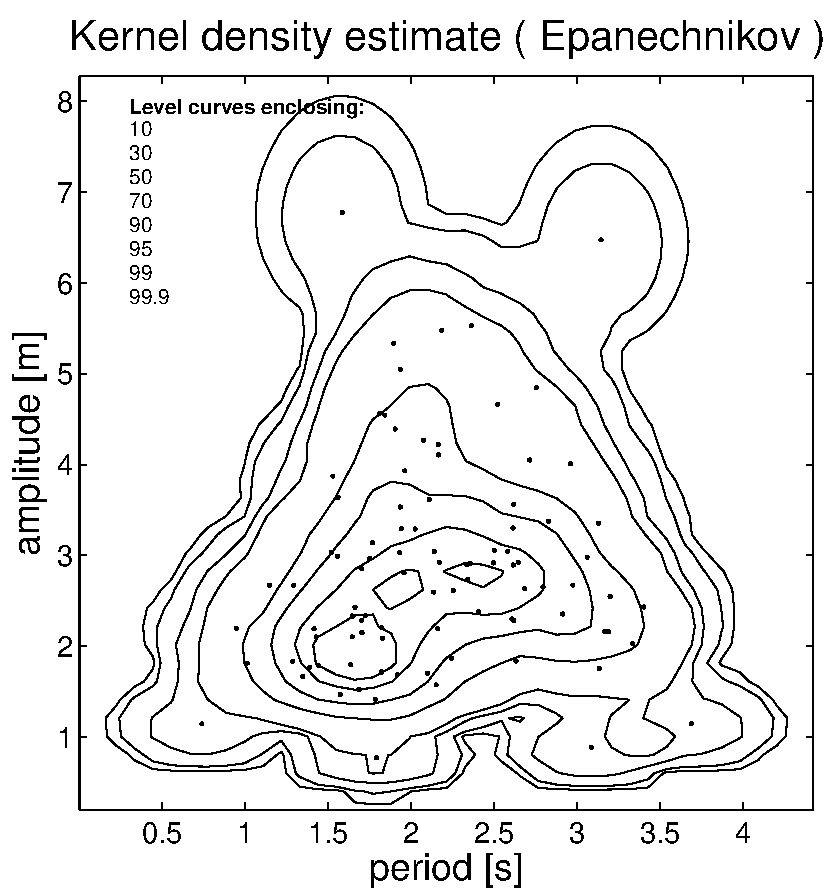
\includegraphics[width=\defwidth]{fig7_6}
\end{minipage}}%
\hfill
\subfigure[]{%
\begin{minipage}[b]{0.5\textwidth}%
\centering 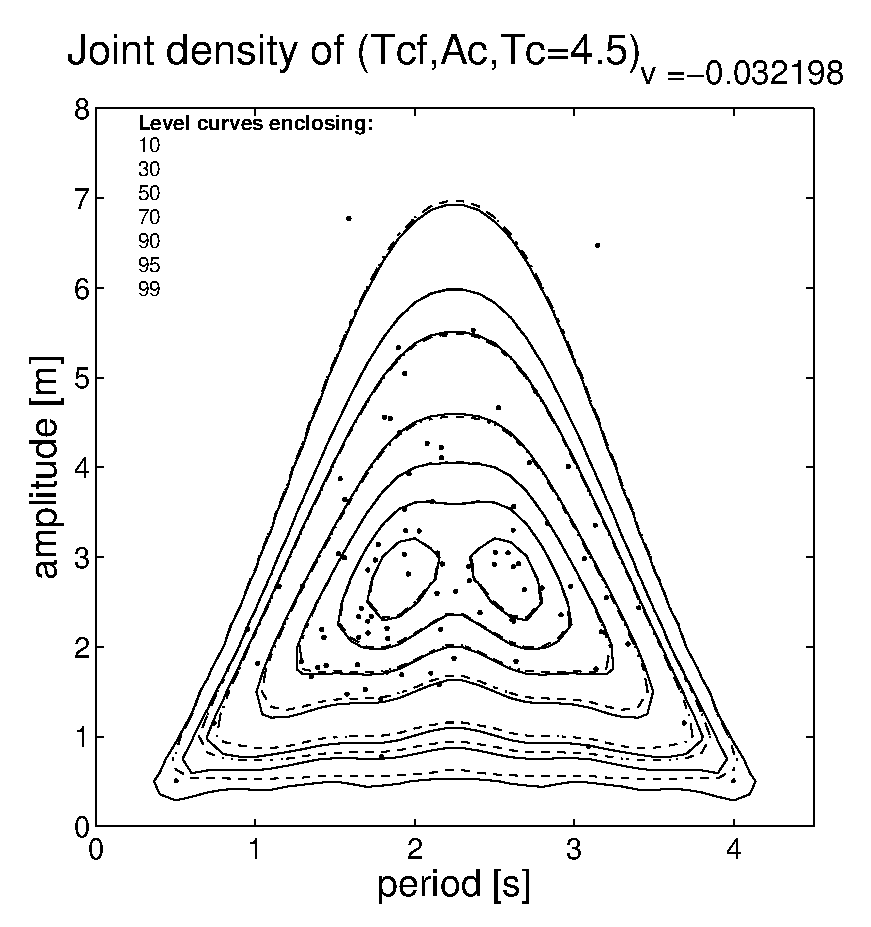
\includegraphics[width=\defwidth]{fig7_7}
\end{minipage}}
\vspace{-3mm}
  \caption[Estimated density of crest position and height compared
  with data]{
Distribution of crest position and crest height for Gullfaks waves with crest period
{\tt Tc = 4.5[s]}.
(a) The estimated (KDE) density of crest position and
    height together with observations (dots). (b) The theoretically
    computed density with {\tt nit = -1, 2} and the data.
}
 \label{fig76}
\end{figure}

In Figure~\ref{fig76}(a) the estimated (KDE) joint density is given
and it should be compared with Figure~\ref{fig76}(b), where the
theoretical density is presented. Here we can really see the advantage
of the theoretically computed densities. Even if we have here used a
long record of wave data, there is not enough of waves to make a
reliable estimate of the joint density, and in a standard 20 minutes
records there would be far too few observations.
\end{cex}

As we have mentioned already the  integral over the crest position of the
computed densities is equal to the joint density of crest period and
height. So in order to get the whole density of {\tt Tc, Ac} one
needs to execute the previous program to obtain the density of
{\tt Tc, Tcf, Ac}  for different values of {\tt Tc} and integrate out
the variable  {\tt Tcf}, and this will take some time.  However, 
most time is spent on the computation of the density of long and small
waves, and these are not interesting. Hence we can start to compute the
joint density of {\tt Tc,Ac} for significant waves.

\begin{cex}{Ex_preliminary_analysis}{\sl (Joint crest period/amplitude for significant waves)} 
 We compute the joint density of
\verb+Tc,Ac+ of significant waves in the Gullfaks data in order to
compare the distribution with the Longuet-Higgins approximation; see
Section~\ref{sec:explicit_approximations}. The following call takes
substantial time (35 minutes), and gives the ``exact'' distribution.
It is not included in the ``fast'' version of the command file {\tt
  Chapter4.m}. 
{\small\begin{verbatim}
      f_tcac_s = spec2thpdf(SG,[],'TcAc',[0 12 81],[Hs/2:0.1:2*Hs],opt1);
\end{verbatim}
}

Next, we find the modified Longuet-Higgins density, i.e.\
the density with transformed crest heights.
The original LH-density underestimates the high crests
with up to one meter.  We can see that for significant waves and
the present spectrum the modified Longuet-Higgins density is quite accurate.
{\small\begin{verbatim}
      mom = spec2mom(SS,4,[],0);
      t = f_tcac_s.x{1}; h = f_tcac_s.x{2};
      flh_g = lh83pdf(t',h',[mom(1),mom(2),mom(3)],SS.tr);
      ind = find(Ac>Hs/2);
      plot(Tc(ind), Ac(ind),'.'); hold on
      pdfplot(flh_g,'k-.');  pdfplot(f_tcac_s); hold off
\end{verbatim}
} \index[xcmds]{{\tt lh83pdf}}

\noindent
In Figure~\ref{fig77}(a) the theoretical density is plotted with solid
lines and the transformed LH-density with dash dotted lines.
We can see that the simple approximation is working very well,
even if it gives slightly too short periods.
%%%%%%%%%%%%%%%%%%%%%%%%%%%%%%%%%%%%%
\begin{figure}[tbh]
\subfigure[]{%
\begin{minipage}{0.5\textwidth}
\centering 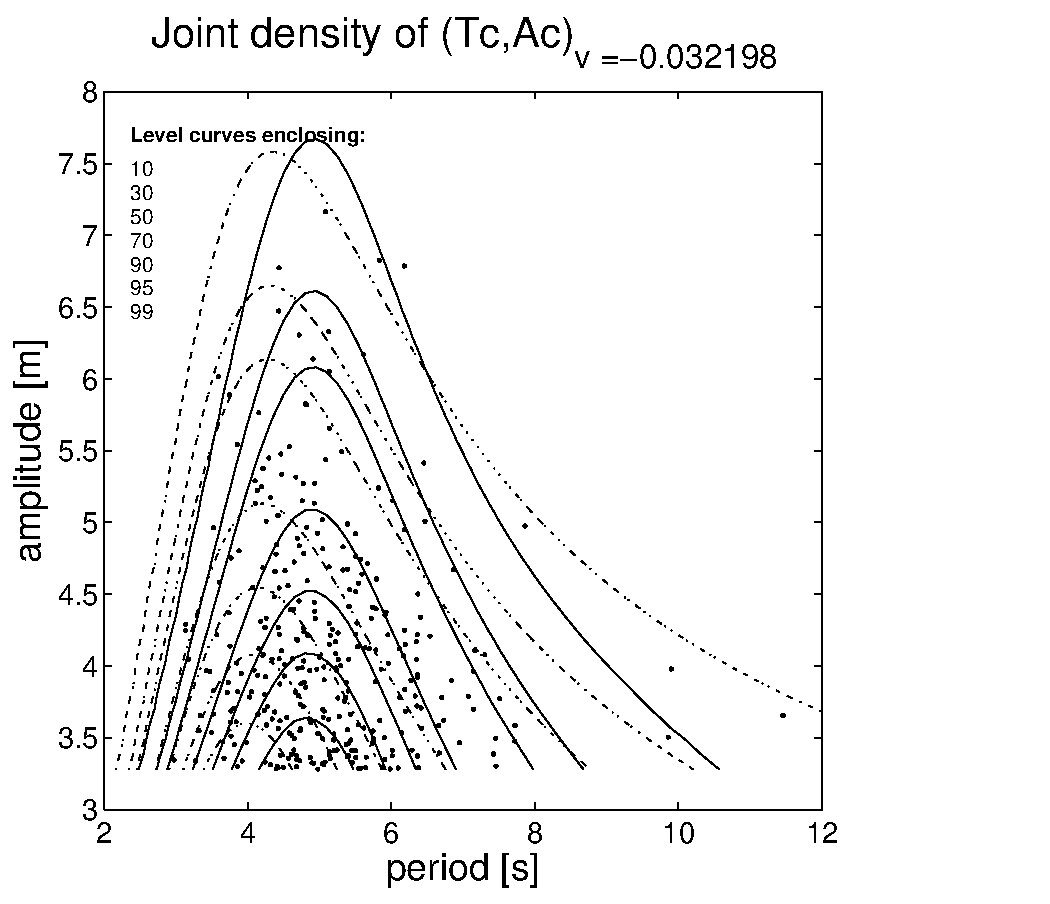
\includegraphics[width=\narrowfigwidth]{fig7_8_2017}
%\centering 
%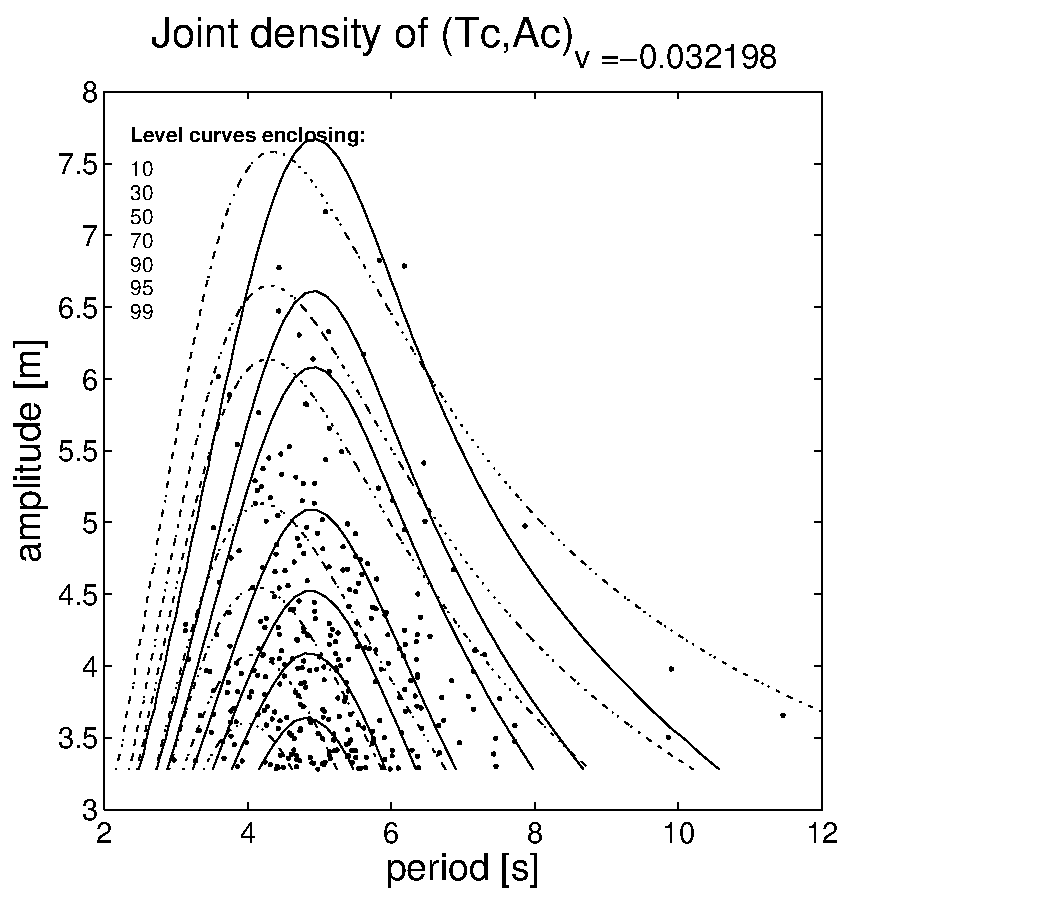
\includegraphics[width=0.45\textwidth]{fig7_8}
\end{minipage}}
\hfill
\subfigure[]{%
\begin{minipage}{0.5\textwidth}%
\centering 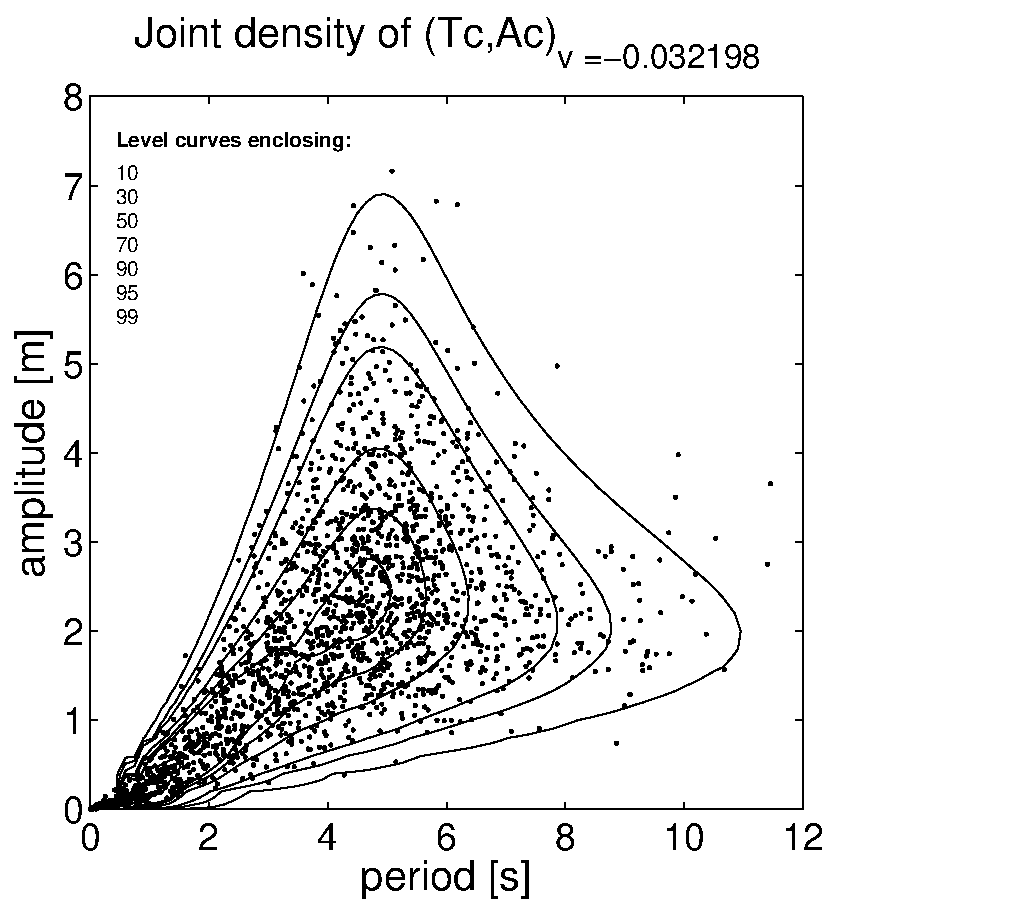
\includegraphics[width=\narrowfigwidth]{fig7_9_2017}
\end{minipage}}
\vspace{-3mm}
\caption[Joint density of {\tt Tc} and {\tt Ac}
compared with Longuet-Higgins density]{
Joint density of {\tt Tc} and {\tt Ac} for the transformed
Gaussian model of the sea measurements from Gullfaks C platform (solid
line) compared with the transformed Longuet-Higgins density (dash
dotted line) and the data (dots) for waves with significant crest.
}
  \label{fig77}
\end{figure}

Finally, we compute the density for all wave heights.
{\small\begin{verbatim}
      f_tcac = spec2thpdf(SG,[],'TcAc',[0 12 81],[0:0.2:8],opt1);
      pdfplot(f_tcac)
\end{verbatim}
}
In
Figure~\ref{fig77}(b) the theoretical density is compared with the
data, and as we see, the agreement is again quite good.
This routine take about 15~minutes to run, and it is not executed in the
default version of the command file {\tt Chapter4.m}.
\end{cex}
\index[xentr]{wave distributions!computation of densities!
joint crest height/period|)}

\subsection{Joint density of crest height and trough depth}

\index[xentr]{wave distributions!computation of densities!
joint crest/trough height|(}

In previous sections we presented programs that compute joint
densities of different  wave characteristics. We started with marginal
densities of crest and trough periods {\tt Tc, Tt}, and then the joint
density of  {\tt Tc,Tt} was derived in order to get the full wave
period {\tt Tu}. Next, we considered {\tt Tc,Tcr,Ac}, crest period,
crest position, and crest height. (The same is possible for
{\tt Tt,Ttb,At}.)
However, in order to fully describe a wave we should
compute the joint density of {\tt Tc,Tac,Ac,Tt,Tat,At}. It is
possible to write a program that computes such six dimensional
densities and it would not take more then 10 minutes of computer time
to compute the density for 200, say,  different combinations of the
characteristics. But in order to describe a six dimensional density
one needs may be 100~000 combinations of values and this is not
practically possible yet.\index[xcmds]{{\tt spec2AcAt}}
Observe that, by numerical differentiation, one can compute the joint
density of {\tt Tc,Ac,Tt,At} using {\tt spec2tccpdf}
(or {\tt spec2AcAt}). This approach is rather time consuming, 
see \cite{LindgrenAndBroberg2004Cycle}.
% but it would take many hours to do such computations. 

There are however some alternatives. From previous studies we know
that very high crests (troughs) occur at the local maximum (minimum)
closest to a zero crossing. We also know that it is the
derivative at the crossing that mainly determines the height of the
wave crest. Consequently, the  steepness of a wave is mainly
determined by the height and location of {\it the last minimum before}
and {\it the first maximum after} an upcrossing of the still water
level. This particular type of min-to-max wave is called a {\it mean
  separated minimum-to-maximum} wave. In general, we can introduce a
{\it $v$-level separated min-to-max wave} to be the last minimum
before and the first maximum after a level $v$ upcrossing.
The distance between the mean-level separated minima and maxima,
denoted {\tt TmM} can be used to compute steepness of a wave, see
\cite{Brodtkorb2004Probability,Brodtkorb2006Evaluating} for details.
The function {\tt spec2mmtpdf} computes the joint density of
\verb+v+-separated wave length and other characteristics of the
{\tt v}-separated minima and maxima. It also computes the joint
density of all pairs of local minima, maxima and the distance
in between; see \cite{LindgrenAndBroberg2004Cycle} for examples.
\index[xentr]{wave distributions!computation of densities!
joint crest/trough height|)} \index[xcmds]{{\tt spec2mmtpdf}}

\subsection{Min-to-max distributions -- Markov method}\label{sect3_5}
\index[xentr]{period!min-to-max}
\index[xentr]{wave distributions!computation of densities!
min-to-max amp./period|(}
\index[xentr]{min-to-max!period|(}
\index[xentr]{min-to-max!amplitude|(}

We shall now investigate another wave characteristic, the
min-to-max wave distribution, including the min-to-max period and
amplitude. This requires the joint density of the height of a local
minimum (maximum) and the following maximum (minimum). The \progname{}
routine that handles this is called \verb+spec2mmtpdf+, and
calculates, i.a.\ the joint density of the height of a maximum and
the following minimum; see the help text to \verb+spec2mmtpdf+.

One important application of the min-to-max distribution is for
approximation of the joint density of {\tt Ac,At}, the crest and
trough amplitudes, by approximating the sequence of local extremes in
a transformed Gaussian model by a Markov chain; see
\cite{RychlikEtal1997Modelling} for
detailed description of the algorithm. The approximation has been
checked on many different sea data giving very accurate results, and it
is also relatively fast.
There is another program {\tt spec2cmat}\index[xcmds]{{\tt spec2cmat}} which  
is somewhat less accurate but even faster.
It is used in Chapter~\ref{cha:5} to compute Markov matrices and rainflow
matrices used in fatigue.

\begin{figure}[tbh]
\centering  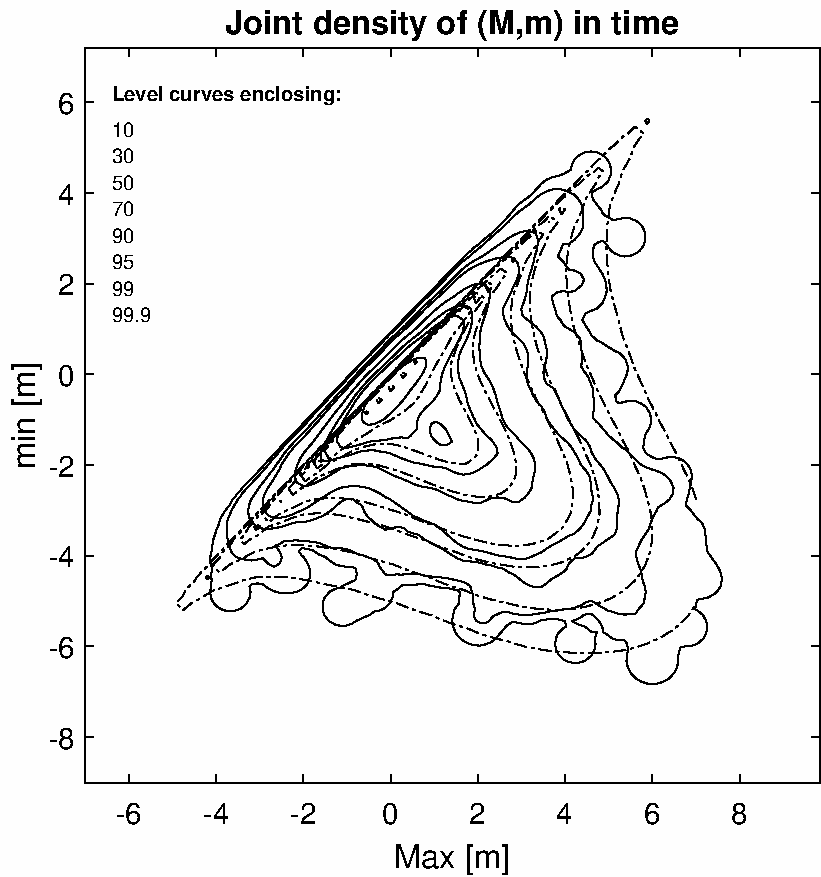
\includegraphics[height=80mm]{fig7_10_2017}
%\centering  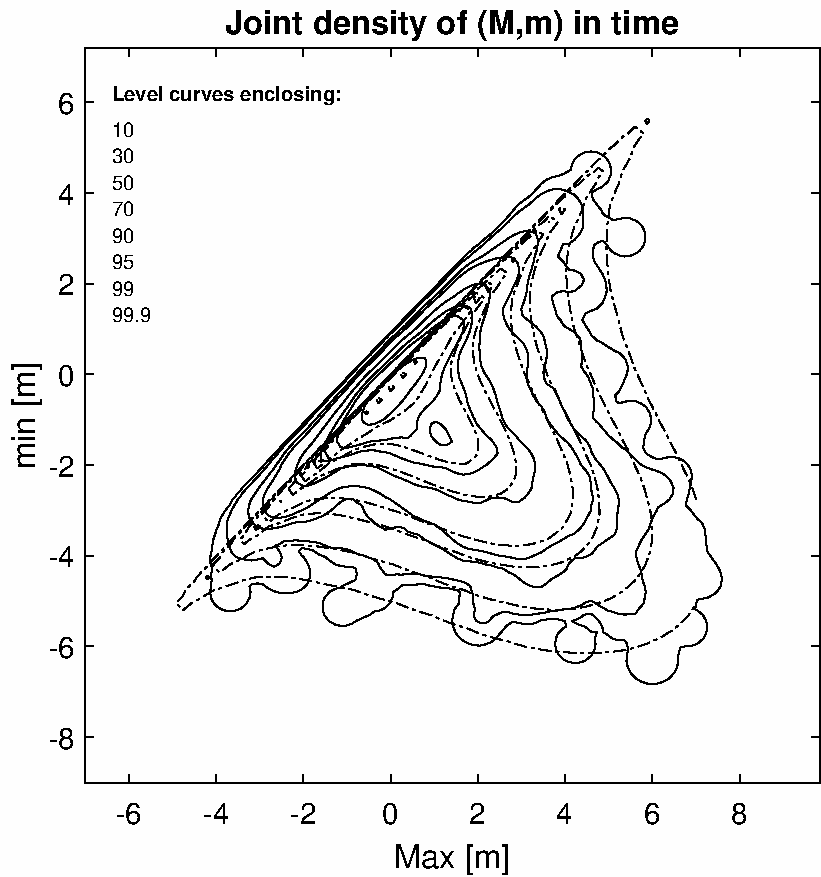
\includegraphics[width=\onefigwidth]{fig7_10_2017}
\vspace{-3mm}
  \caption[Joint density of maximum and minimum for Gullfaks~C
data]{
Joint density of maximum and the following minimum for the
transformed Gaussian model of the sea measurements from Gullfaks~C 
(dash-dotted lines) compared with the estimated (KDE)
density from data (solid lines).
}
  \label{fig78}
\end{figure}

\begin{rtex}{Gullfaks_min_max}{min-max problems with Gullfaks data}
In this example we continue the analysis of the  Gullfaks~C platform
data. First we shall retrieve the sequence of turning points, i.e.\ the
minima and maxima, in {\tt yy} and calculate the theoretical distribution.
{\small\begin{verbatim}
      opt2 = rindoptset('speed',5,'nit',2,'method',0);
      tp = dat2tp(yy);
      Mm = fliplr(tp2mm(tp));
      fmm = kde(Mm);
      f_mM = spec2mmtpdf(SG,[],'mm',[],[-7 7 51],opt2);
      pdfplot(f_mM,'-.'), hold on
      pdfplot(fmm,'k-'), hold off
\end{verbatim}
}
In Figure~\ref{fig78} we can see that the theoretically computed density
agrees very well with the estimated one,
even with an as low a {\tt nit} as 2.
\end{rtex}
\index[xcmds]{{\tt spec2mmtpdf}}
\index[xcmds]{{\tt rindoptset}}

\begin{rtex}{Crest-trough-from-min-max}{Crest-trough distribution from
min-max transitions}
We turn now to the joint density of crest and trough. We first
compute the exact distribution with the help of \verb+spec2mmtpdf+,
and then compare the result with that obtained by means of the Markov
approximation for the stillwater-separated
min-max sequence; see Section~\ref{subsec:markov_chain}.
{\small\begin{verbatim}
      ind = find(Mm(:,1)>v && Mm(:,2)<v);
      Mmv = abs(Mm(ind,:)-v);
      fmmv = kde(Mmv,'epan');
      f_vmm = spec2mmtpdf(SG,[],'vmm',[],[-7 7 51],opt2);
      pdfplot(fmmv,'k-'), hold on
      pdfplot(f_vmm,'-.'), hold off
\end{verbatim}}
\noindent
Then we compute the joint density of crest and trough
using the Markov approximation to the sequence of local
extremes (sequence of turning points {\tt tp}).
{\small\begin{verbatim}
      facat = kde([Ac At]);
      f_acat = spec2mmtpdf(SG,[],'AcAt',[],[-7 7 51],opt2);
      pdfplot(f_acat,'-.'), hold on
      pdfplot(facat,'k-'), hold off
\end{verbatim}
}

\begin{figure}[tbh]
\subfigure[]{%
\begin{minipage}[b]{0.5\textwidth}%
\centering 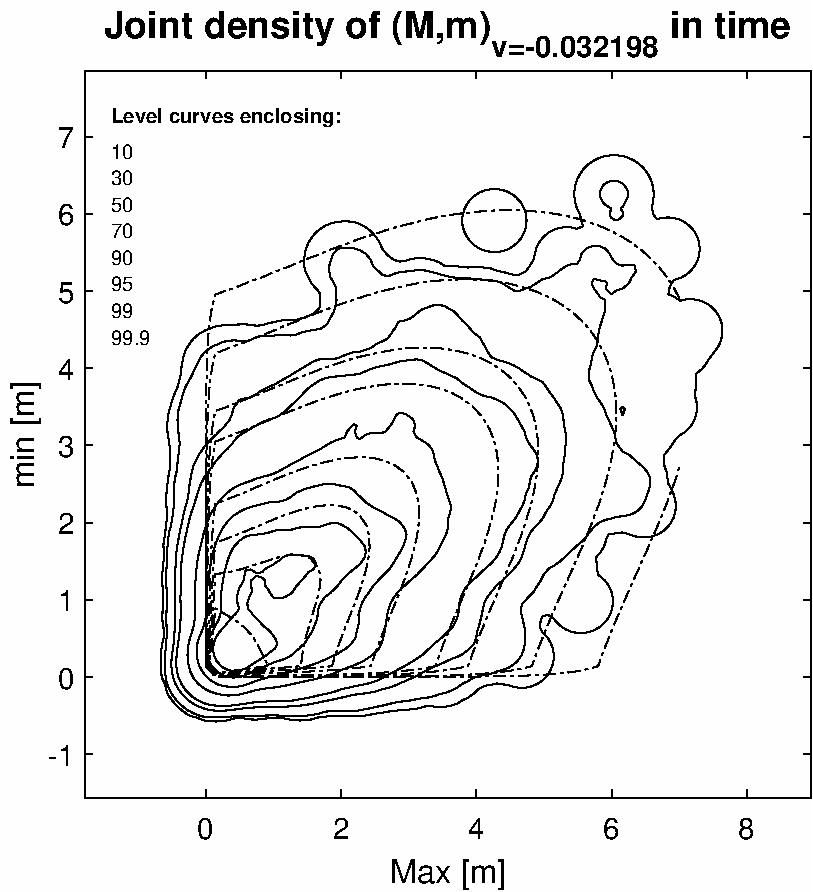
\includegraphics[height=60mm]{fig7_11_2017}
\end{minipage}}%
\hfill
\subfigure[]{%
\begin{minipage}[b]{0.5\textwidth}%
\centering 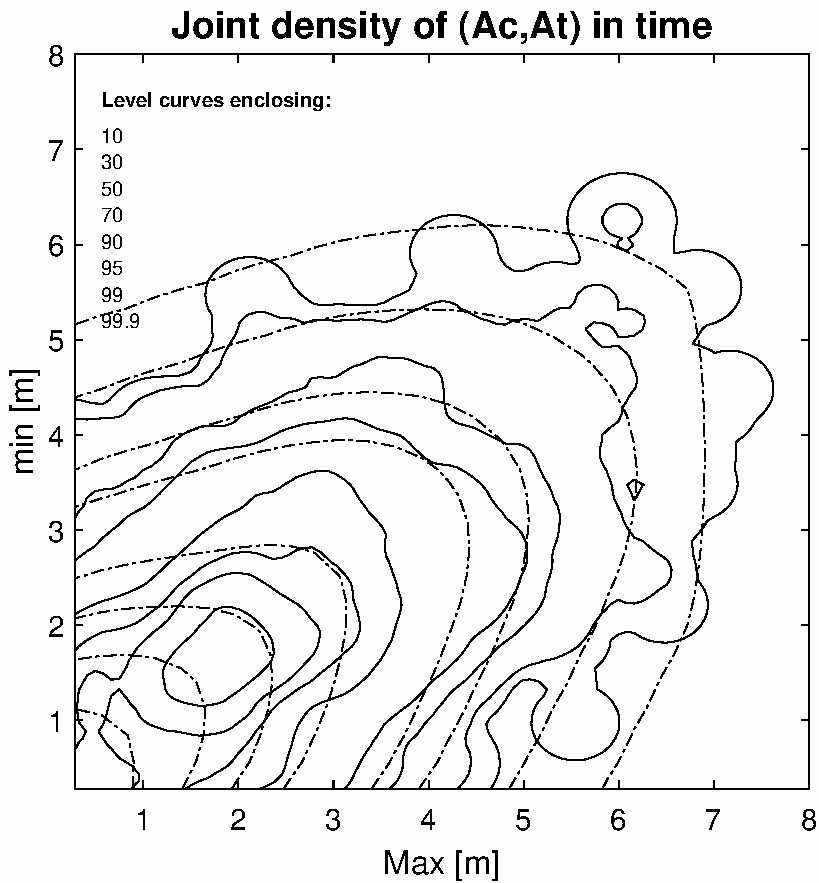
\includegraphics[height=60mm]{fig7_12_2017}
\end{minipage}}
\vspace{-3mm}
  \caption[Pdf of stillwater-separated
min-to-max values for Gullfaks~C data]{
Estimated joint density (KDE) of  stillwater-separated
min-to-max values for the
measurements from Gullfaks~C (solid line) compared with:
(a) the transformed Gaussian model for the
measurements (dash-dotted line).
(b) Markov approximation for the joint density of crest and trough
height {\tt Ac,At} (dash-dotted line).
}
  \label{fig79}
\end{figure}

Now we are in the position to check our two methods, the Markov
method, where the min-to-max sequence is approximated by a Markov
chain, and the replacement of the true min-to-max transition
probabilities by the transition probabilities that are valid for the
stillwater-separated min-to-max values. The results are presented
in Figure~\ref{fig79}. We see in (a) that the stillwater-separated
min-to-max distribution miss a considerable number of min-to-max
values, which fall on the same side of the still water level. On the
other hand, figure (b) indicates that
the Markov assumption is acceptable.
\end{rtex}


\index[xentr]{wave distributions!computation of densities!
min-to-max amp./period|)}
\index[xentr]{min-to-max!period|)}
\index[xentr]{min-to-max!amplitude|)}

\newpage
\section{\progname{} wave characteristics routines}
\label{s:waveroutines}

{\small\begin{verbatim}
help trgauss

 Module TRGAUSS in WAFO Toolbox.
 Version 2.5.2   07-Feb-2011

 Readme          - New features, bug fixes, and changes in TRGAUSS.

 Misc
   createpdf     - PDF struct constructor.
   pdfplot       - Plot contents of pdf structures.
   trplot        - Plots transformation, g, eg. estimated with dat2tr.

 Transforms and non-linearities
   dat2gaus      - Transforms  x  using the transformation  g.
   gaus2dat      - Transforms  xx  using the inverse of  g.
   testgaussian  - Test if a stochastic process is Gaussian.
   spec2skew     - Estimates the moments of 2'nd order non-linear waves.
   trangood      - Makes a transformation that is suitable for
                   efficient transforms.
   tranproc      - Transforms process X and up to four derivatives.
   trmak         - Put together a transformation object.
   troptset      - Create or alter TRANSFORM OPTIONS structure.
   trunmak       - Split a transformation object into its pieces.

 Transformed Gaussian model estimation
   cdf2tr        - Estimate transformation, g, from observed CDF.
   dat2tr        - Estimate transformation, g, from data.
   hermitetr     - Estimate transformation, g, from the first 4 moments.
   ochitr        - Estimate transformation, g, from the first 3 moments.
   lc2tr         - Estimate transformation, g, from observed
                   crossing intensity.
   lc2tr2        - Estimate transformation, g, from observed
                   crossing intensity, version 2.

 Gaussian probabilities and expectations
   cdfnorm2d     - Bivariate normal cumulative distribution function.
   prbnorm2d     - Bivariate normal probability.
   prbnormnd     - Multivariate normal probability by Genz' algorithm.
   prbnormndpc   - Multivariate normal probabilities with
                   product correlation.
   prbnormtnd    - Multivariate normal or T probability by
                   Genz' algorithm.
   prbnormtndpc  - Multivariate normal or T probability with
                   product correlation structure.
   rind          - Computes multivariate normal expectations.
   rindoptset    - Create or alter RIND OPTIONS structure.

 Probability density functions (pdf) or intensity matrices
   chitwo2lc_sorm - SORM-approximation of crossing intensity,
                    noncentral Chi^2 process.
   chitwo2lc_sp  - Saddlepoint approximation of crossing
                   intensity, noncentral Chi^2 process.
   dirsp2chitwo  - Parameters in non-central CHI-TWO process for
                   directional Stokes waves.
   iter          - Calculates a Markov matrix given a rainflow matrix.
   iter_mc       - Calculates a kernel of a MC given a rainflow matrix.
   mc2rfc        - Calculates a rainflow matrix given a
                   Markov chain with kernel f_xy.
   mctp2rfc      - Rainflow matrix given a Markov matrix of a
                   Markov chain of turning points.
   mctp2tc       - Calculates frequencies for the upcrossing
                   troughs and crests.
   nt2fr         - Calculates the frequency matrix given the
                   counting distribution matrix.
   spec2cmat     - Joint intensity matrix for cycles (max,min)-,
                   rainflow- and (crest,trough).
   spec2mmtpdf   - Joint density of Maximum, minimum and period.
   spec2tccpdf   - Density of crest-to-crest
                   wave-period or -length.
   spec2thpdf    - Joint density of amplitude and
                   period/wave-length characteristics.
   spec2tpdf     - Density of crest/trough- period or length.
   spec2tpdf2    - Density of crest/trough- period or length,
                   version 2.
   specq2lc      - Saddlepoint approximation of crossing
                   intensity for quadratic sea.
   th2vhpdf      - Transform joint T-H density to V-H density.

 Cumulative distribution functions (cdf)
   cdflomax      - CDF for local maxima for a zero-mean
                   Gaussian process.
   spec2AcAt     - Survival function for crests and troughs,
                   R(h1,h2)=P(Ac>h1,At>h2).
   spec2Acdf     - CDF for crests P(Ac<=h) or troughs P(At<=h).
\end{verbatim}

%%% Local Variables:
%%% mode: latex
%%% TeX-master: "wafomanual"
%%% End:
